\documentclass[11pt,a4paper]{article}

% -- Encoding & Fonts --
\usepackage[utf8]{inputenc}
\usepackage[T1]{fontenc}
\IfFileExists{lmodern.sty}{\usepackage{lmodern}}{}

% -- Mathematics --
\usepackage{amsmath,amssymb,amsthm,mathtools}

% -- Layout --
\usepackage[margin=2.5cm]{geometry}
\usepackage{setspace}
\doublespacing
\usepackage{parskip}

% -- Line numbers for review --
\IfFileExists{lineno.sty}{%
  \usepackage{lineno}
  \linenumbers
}{}

% -- Section formatting --
\usepackage{titlesec}
\titleformat{\section}{\large\bfseries}{\thesection.}{0.5em}{}
\titleformat{\subsection}{\normalsize\bfseries}{\thesubsection}{0.5em}{}
\titleformat{\subsubsection}{\normalsize\itshape}{\thesubsubsection}{0.5em}{}

% -- Headers & footers --
\usepackage{fancyhdr}
\pagestyle{fancy}
\fancyhf{}
\fancyhead[L]{\small\textit{Balanced-coherence regimes for neural access}}
\fancyhead[R]{\small\textit{Tugan}}
\fancyfoot[C]{\thepage}
\renewcommand{\headrulewidth}{0.4pt}

% -- Hyperlinks --
\usepackage{xcolor}
\usepackage[colorlinks=true,linkcolor=black,citecolor=black,urlcolor=black]{hyperref}

% -- Bibliography --
\usepackage[numbers,sort&compress]{natbib}

\usepackage{graphicx}
\graphicspath{{submission_figures/}}
\IfFileExists{booktabs.sty}{%
  \usepackage{booktabs}
}{%
  \newcommand{\toprule}{\hline}
  \newcommand{\midrule}{\hline}
  \newcommand{\bottomrule}{\hline}
}

% -- Theorem environments --
\theoremstyle{plain}
\newtheorem{theorem}{Theorem}[section]
\newtheorem{proposition}[theorem]{Proposition}
\newtheorem{corollary}[theorem]{Corollary}
\theoremstyle{definition}
\newtheorem{definition}[theorem]{Definition}
\theoremstyle{remark}
\newtheorem*{remark}{Remark}
\newtheorem*{significance}{Significance}

% -- Custom commands --
\newcommand{\Deff}{D_{\mathrm{eff}}}
\newcommand{\Mtau}{M_{\tau}}
\newcommand{\Rmin}{R_{\min}}
\newcommand{\Dmin}{D_{\min}}
\newcommand{\Dmax}{D_{\max}}
\newcommand{\Mmin}{M_{\min}}
\newcommand{\Mmax}{M_{\max}}
\newcommand{\Gmax}{G_{\max}}
\newcommand{\Kcop}{K_c^{\mathrm{op}}}
\newcommand{\Lobs}{L_{\mathrm{obs}}}

\title{%
  \textbf{Balanced-coherence regimes of conscious access: a computational model with public EEG validation}
}
\author{%
  Mehmet Oktay Tugan\textsuperscript{1,*}
}
\date{}

% ==================================================================
\begin{document}
\maketitle
\thispagestyle{fancy}

\noindent
\textsuperscript{1} Independent Researcher, Zurich, Switzerland

\noindent
ORCID: 0009-0005-8665-3583

\noindent
\textsuperscript{*} Corresponding author: oktaytugan82@gmail.com

\medskip
\noindent
\textbf{Short title:} Balanced-coherence regimes for neural access

\bigskip

% -- Abstract --
\begin{abstract}
\noindent
The Gamma-Code Consensus (GCC) is a computational model of conscious-access-compatible dynamics. It proposes that global access is not maximized by synchrony alone, but by a bounded regime in which coherence, effective dimensionality, and temporal variability jointly remain within calibrated ranges. We formalize this regime in a stochastic phase-oscillator network with separable topology, global gain, and population-specific efficacy, then derive six falsifiable predictions. Synthetic network simulations reproduce the evaluated prediction family: nonlinear thresholding, degradation-dependent threshold shifts, bounded access intervals, anesthesia-like trajectories, and selective-preservation re-entry under controlled assumptions. Public EEG analyses provide convergent but deliberately limited empirical support. In Chennu et al.\ 2016 ($N=20$), the subject-calibrated access index declines under propofol sedation and survives fsaverage template-source reconstruction. In OpenNeuro DS005620 ($N=20$ paired), the same direction replicates, and frozen cross-dataset gamma benchmarks generalize above chance, including a wPLI-based lagged-coupling variant. Sleep-EDF ($22$ recordings) shows cross-paradigm state geometry: GCC triad features separate Wake/NREM and REM/NREM, although spectral sleep features remain stronger. A public disorders-of-consciousness EEG/PSG dataset provides a pilot clinical anchor: alpha-band GCC distinguishes MCS+ from VS and remains positive after spectral and retained-epoch residualization. Spectral controls show that GCC is not a bandpower-independent biomarker. The present contribution is therefore a theory-guided, empirically stress-tested regime model of access-compatible dynamics; the stronger clinical hypothesis of selective re-entry in structurally degraded brains remains a future target.
\end{abstract}

\medskip
\noindent\textbf{Keywords:} consciousness; global access; EEG; propofol; disorders of consciousness; metastability; phase synchronization; computational neuroscience

\newpage

% ==================================================================
% ======================= INTRODUCTION =============================
% ==================================================================
\section*{Introduction}
\addcontentsline{toc}{section}{Introduction}

% ==================================================================
\section{Aim and Scope}
\label{sec:ziel}

The GCC is a principled model of level of consciousness and global access. It asks when a heterogeneous, noisy, and degradable network enters an integrated but non-rigid macroscopic regime. It is not a theory of qualia; it is a regime model related to global-access, integration/differentiation, metastability, perturbational-complexity, and clinical state-marker approaches \citep{dehaene1998,tononi2004,fries2015,deco2017,casali2013,sitt2014,engemann2018,demertzi2019,mashour2020}.

The evaluated core claim is that access-compatible dynamics occupy a bounded region jointly characterized by coherence, effective dimensionality, and temporal variability. This claim generates predictions P2--P6 and is tested through synthetic simulations and public EEG/PSG analyses. A narrower degradation extension concerns selective re-integration in damaged systems:

\begin{quote}
\itshape
In degraded neural systems, global access can arise not only from increased activity but also from selective collapse of competing parts of the network. Functional re-integration then follows from gain redistribution onto a residual backbone structure, rather than from a global energy surge.
\end{quote}

This extension is conditional: it concerns degraded systems near the lower edge of the access region, not healthy systems already stably within it. Its empirical consequence is prediction~P1, but direct biological validation of P1 is not claimed here.

\paragraph{Three-stage evaluation.}
The paper tests model-internal consistency in synthetic Kuramoto networks, applies the observables to public propofol EEG datasets plus sleep, ketamine, DoC, and dementia-proxy checks, and benchmarks GCC against spectral, artifact, lagged-coupling, phase-only, source-proxy, and reliability controls. These analyses establish operational state sensitivity, not direct selective-preservation validation in structurally degraded brains.


% ==================================================================
\section{Core Intuition}
\label{sec:intuition}

The model assumes that conscious access is favoured neither by maximal desynchronization nor by maximal synchronization. Too little coordination prevents global integration; too much rigid coordination collapses the dynamics onto few inflexible modes. The favourable range lies between these extremes, where global coordination, reduced but not collapsed dimensionality, and temporal variability co-occur \citep{fries2015,deco2017}.

The core regime claim is therefore not ``consciousness is synchrony'' but:

\begin{quote}
\itshape
Level of consciousness and global access arise in a regime of balanced consensus formation within a noisy, heterogeneous network.
\end{quote}


% ==================================================================
\section{Core Dynamical Model}
\label{sec:core}
\label{sec:kernmodell}

We model $N$ neural populations as phase oscillators on a weighted network. The dynamics of population~$i$ is given by

\begin{equation}
\label{eq:dynamics}
\mathrm{d}\theta_i(t)
= \biggl[\,\omega_i
+ K \cdot G(t) \cdot g_i(t) \sum_{j} W_{ij}(t)\,\sin\!\bigl(\theta_j(t) - \theta_i(t) - \varphi_{ij}(t)\bigr)
\biggr]\,\mathrm{d}t
+ \sigma_i(t)\,\mathrm{d}B_i(t)
\end{equation}

where:
\begin{itemize}
  \item $\theta_i(t)$: phase of population~$i$
  \item $\omega_i$: intrinsic frequency
  \item $K$: global coupling scale
  \item $G(t) > 0$: global gain or excitability factor
  \item $g_i(t) \in [0,1]$: population-specific preservation factor of afferent efficacy
  \item $W_{ij}(t) \geq 0$: normalized residual topology
  \item $\varphi_{ij}(t)$: effective phase delays
  \item $\sigma_i(t) \geq 0$: population-specific noise amplitude
  \item $B_i(t)$: independent standard Brownian motions
\end{itemize}

The matrix~$W(t)$ is obtained from a raw residual adjacency~$A(t)$ by row normalization:

\begin{equation}
\label{eq:normierung}
W_{ij}(t) = \frac{A_{ij}(t)}{m_i(t)}, \qquad m_i(t) = \sum_j A_{ij}(t),
\end{equation}

provided $m_i(t) > 0$; otherwise $W_{ij}(t) = 0$.

The key structural move is the separation of topology~$W$, global excitability~$G$, local preservation~$g_i$, and noise~$\sigma_i$. Row normalization makes incoming structure comparable but would otherwise mask structural loss; $g_i$ retains that loss explicitly. The phase-oscillator framework follows established work on synchronization thresholds in heterogeneous networks \citep{restrepo2005}.


% ==================================================================
\section{Degradation as Topology and Gain Loss}
\label{sec:abbau}
\label{sec:degradation}

The GCC does not model degradation as pure edge removal. Structural and functional damage are separated as:

\begin{enumerate}
  \item $A(t)$ or $W(t)$ describes which connections are topologically preserved.
  \item $g_i(t)$ describes how strongly the remaining inputs remain functionally effective.
\end{enumerate}

A simple working definition is

\begin{equation}
\label{eq:gain}
g_i(t) = \frac{m_i(t)}{m_i^{\mathrm{ref}}},
\end{equation}

where $m_i^{\mathrm{ref}}$ denotes reference incoming mass and $m_i(t)$ current preserved mass. Thus row normalization of $W(t)$ does not erase afferent loss, which remains encoded in $g_i(t)$.

For degenerative conditions, the model takes the defensive form:

\begin{quote}
\itshape
In families of degraded networks, the operational access threshold typically shifts toward higher effective coupling, higher gain, or more favourable noise conditions.
\end{quote}

This is a model-internal, empirically testable tendency, not an unconditional universal claim.


% ==================================================================
% ===================== MATERIALS AND METHODS ======================
% ==================================================================
\section*{Materials and Methods}
\addcontentsline{toc}{section}{Materials and Methods}

% ==================================================================
\section{Three Operational Observables}
\label{sec:observablen}

\subsection{Global Coherence}

\begin{equation}
\label{eq:R}
R(t) = \frac{1}{N}\,\biggl|\sum_{j} e^{i\,\theta_j(t)}\biggr|
\end{equation}

$R(t)$ measures macroscopic phase coherence. It is necessary for coordination but insufficient on its own, because rigid pathological coherence and flexible integration must be distinguished.

\subsection{Effective Dimensionality}

For a window of length~$\tau_D$, define the centred activity

\begin{equation}
X_i(s) = \cos\!\bigl(\theta_i(s)\bigr) - \bigl\langle\cos(\theta_i)\bigr\rangle_{[t-\tau_D,\,t]}
\end{equation}

and the unregularized window covariance matrix $\hat{C}_D(t) = \mathrm{Cov}(X_1,\ldots,X_N)$. To avoid numerical problems in low-rank states, we use a scaled ridge regularization:

\begin{equation}
\label{eq:ridge}
\varepsilon_D^{\lambda}(t) = \max\!\biggl(\lambda\,\frac{\mathrm{tr}\bigl(\hat{C}_D(t)\bigr)}{N},\;\varepsilon_{\mathrm{floor}}\biggr),
\end{equation}

with a dimensionless parameter $\lambda > 0$ and an absolute floor $\varepsilon_{\mathrm{floor}} > 0$. The regularized covariance matrix is

\begin{equation}
C_D^{\lambda}(t) = \hat{C}_D(t) + \varepsilon_D^{\lambda}(t)\cdot I.
\end{equation}

The effective dimensionality is then the participation ratio:

\begin{equation}
\label{eq:Deff}
\boxed{\;\Deff^{\lambda}(t) = \frac{\bigl[\mathrm{tr}\,C_D^{\lambda}(t)\bigr]^2}{\mathrm{tr}\!\bigl[\bigl(C_D^{\lambda}(t)\bigr)^2\bigr]}\;}
\end{equation}

Small values indicate compression onto few modes; large values indicate distributed activity. The relevant range lies between fragmentation and rigid collapse.

\subsection{Temporal Variability (Metastability)}

For a window~$\tau_M$ define:

\begin{equation}
\label{eq:Mtau}
\Mtau(t) = \mathrm{Var}\!\bigl(\,R(s) : s \in [t - \tau_M,\, t]\,\bigr)
\end{equation}

$\Mtau$ measures temporal variability of global coherence. It becomes interpretable only together with $R$ and $\Deff$.


% ==================================================================
\section{Operational Access Region}
\label{sec:access-region}
\label{sec:zugang}

The GCC does not define an ontological criterion for consciousness but an operational access region in the space of observables. Relative to a pre-specified calibration, window choice, and regularization, a system is internally deemed \emph{access-compatible} if

\begin{equation}
\label{eq:zugang}
\boxed{\;
R(t) > \Rmin, \quad
\Dmin < \Deff^{\lambda}(t) < \Dmax, \quad
\Mmin < \Mtau(t) < \Mmax
\;}
\end{equation}

These inequalities are not a metaphysical definition of consciousness. They are a data- and scale-relative working description of a dynamical range favourable for global access.

\subsection{Multiscale Robustness Formulation}

Let $\mathcal{T}_D$, $\mathcal{T}_M$, and $\Lambda$ be finite sets of admissible window lengths and ridge parameters, respectively. For each triple $(\tau_D, \tau_M, \lambda)$ define the indicator

\begin{equation}
\mathcal{A}(t;\,\tau_D,\tau_M,\lambda) =
\begin{cases}
1, & \text{if all three inequalities~\eqref{eq:zugang} are satisfied,}\\
0, & \text{otherwise.}
\end{cases}
\end{equation}

The multiscale access index is

\begin{equation}
\label{eq:Pi}
\Pi(t) = \frac{1}{|\mathcal{T}_D|\,|\mathcal{T}_M|\,|\Lambda|}\,\sum \mathcal{A}(t;\,\tau_D,\tau_M,\lambda).
\end{equation}

A state is window-robustly access-compatible if $\Pi(t) \geq q^*$ for a pre-specified fraction $q^*$.

\subsection{Data-Driven Calibration of Regime Boundaries}

Regime boundaries are estimated from a reference ensemble~$\mathcal{H}$ of access-compatible segments. For a pre-chosen $\alpha \in (0,\,0.5)$:

\begin{align}
\Rmin &= Q_{\alpha}(R \mid \mathcal{H}), \notag\\
\Dmin &= Q_{\alpha}(\Deff^{\lambda} \mid \mathcal{H}), \qquad
\Dmax = Q_{1-\alpha}(\Deff^{\lambda} \mid \mathcal{H}), \label{eq:kalib}\\
\Mmin &= Q_{\alpha}(\Mtau \mid \mathcal{H}), \qquad\;\;
\Mmax = Q_{1-\alpha}(\Mtau \mid \mathcal{H}). \notag
\end{align}

\subsection{Two Positive Reference Levels: $\mathcal{H}_{\mathrm{full}}$ and $\mathcal{H}_{+}$}

For degradation analyses, GCC distinguishes two positive reference levels:

\begin{itemize}
\item $\mathcal{H}_{\mathrm{full}}$: healthy or near-healthy access segments with high macroscopic integration.
\item $\mathcal{H}_{+}$: broader positive ensemble including partial access segments (mildly sedated, mildly degraded).
\end{itemize}

With an exclusion ensemble~$\mathcal{U}$, this separates two claims:

\begin{itemize}
\item \textbf{full-access-compatible:} $\Pi_{\mathrm{full}}(t) \geq q_{\mathrm{full}}$
\item \textbf{partial-re-entry-compatible:} $\Pi_{+}(t) \geq q_{+}$, even if $\Pi_{\mathrm{full}}(t) < q_{\mathrm{full}}$
\end{itemize}

This prevents partial re-entry from being falsely rejected merely because it is not healthy-like full access.


% ==================================================================
\section{Operational Access Threshold Instead of a Universal~$K_c$}
\label{sec:schwelle}

For finite, noisy, and topologically heterogeneous networks, $K_c$ is not a universal single number. The GCC uses an operational access threshold~$\Kcop$:

\begin{equation}
\label{eq:Kcop}
\Kcop = \operatorname*{arg\,max}_{K}\;\frac{\mathrm{d}\langle R \rangle}{\mathrm{d}K}
\qquad\text{or}\qquad
\Kcop = \operatorname*{arg\,max}_{K}\;\chi_R(K), \quad \chi_R(K) = \mathrm{Var}_t\!\bigl(R(t;K)\bigr).
\end{equation}

The threshold is therefore treated as an observable regime transition rather than an a priori constant \citep{restrepo2005}.


% ==================================================================
\section{Basic Mathematical Properties}
\label{sec:grundsaetze}

Under $W_{ij} \geq 0$, $\sum_j W_{ij} = 1$, and $|\sin(\cdot)| \leq 1$, the deterministic coupling term is bounded:

\begin{equation}
\bigl|K \cdot G(t) \cdot g_i(t) \sum_j W_{ij}(t)\,\sin(\cdots)\bigr| \;\leq\; K \cdot G(t) \cdot g_i(t).
\end{equation}

For the observables the elementary bounds hold:

\begin{equation}
1 \leq \Deff(t) \leq \mathrm{rank}\bigl(C_D(t)\bigr) \leq N,
\end{equation}

If $R(s)$ is constant over the window, then $\Mtau(t)=0$. High coherence alone is therefore insufficient; a rigid state has low metastability.


% ==================================================================
\section{Selective-Preservation Re-Entry as a Degradation Extension}
\label{sec:TL}

The GCC contains a degradation extension: after exit from the access-compatible regime, selective preservation of efficacy on a residual subnetwork may permit transient partial re-entry. This is the most distinctive mechanistic extension, but the evaluated core of the paper is P2--P6 in simulations and public EEG/PSG validation.

Lucidity-like re-entry remains a possible future clinical application, not an empirical result established here.

\subsection{Residual Backbone Structure}

Let $S$ be a representation-relevant population subset. ``Residual'' means not healthy, but connected enough to support a scaffold:

\begin{equation}
\label{eq:backbone}
S(t;\,g_*) = \text{largest connected component of the subgraph on } \{i : g_i(t) \geq g_*\}.
\end{equation}

\subsection{Selective Gain Preservation Instead of a Global Energy Surge}

The proposed extension mechanism is:

\begin{quote}
\itshape
A lucidity-like or re-integration episode, if produced by the GCC mechanism, would not correspond to a global energy surge but to short-term functional concentration of remaining efficacy on a residual backbone structure.
\end{quote}

The effective afferent drive of population~$i$ is proportional to

\begin{equation}
\label{eq:Lambda}
\Lambda_i(t) = K \cdot G(t) \cdot g_i(t).
\end{equation}

Even if $G(t)$ decreases overall, preserved populations can gain relative influence over collapsing populations, yielding temporary residual-backbone reorganization.

\subsection{Three Conditions for a Re-Entry}

Selective-preservation re-entry requires:

\begin{enumerate}
\item \textbf{Structural residual condition:} A residual backbone structure $S$ is still present.
\item \textbf{Gain condition:} For populations in $S$, $\Lambda_i(t)$ remains sufficiently high during a short interval.
\item \textbf{Dynamical admissibility:} Noise, delay dispersion, and frequency spread prevent neither integration nor flexible dynamics.
\end{enumerate}

These conditions are strict; the model does not imply a final clarity episode in every degraded or dying process.

\subsection{What the Model Explicitly Does Not Claim}

The model does \emph{not} claim that terminal or paradoxical lucidity is demonstrated here, that lucidity has a single mechanism, that noise reduction is sufficient, that high coherence explains autobiographical memory, or that dying processes necessarily produce a final consensus-like peak.


% ==================================================================
\section{Predictions}
\label{sec:predictions}
\label{sec:vorhersagen}

P2--P6 form the evaluated prediction family. P1 is retained as a clinical degradation extension, model-internally instantiated by P6 but not biologically validated here.

\medskip
\noindent\textbf{P2.\;Critical range.}\quad
Near the access threshold the system shows non-linear reorganization rather than arbitrary gradual drift.

\medskip
\noindent\textbf{P3.\;Degradation shift.}\quad
In degraded network ensembles, $\Kcop$ shifts toward higher effective coupling or gain.

\medskip
\noindent\textbf{P4.\;Bounded interval.}\quad
Global access is expected in an intermediate range, not at maximal desynchronization or rigid synchrony.

\medskip
\noindent\textbf{P5.\;State trajectories.}\quad
State transitions can be described as motion in the space spanned by $W$, $G$, $g_i$, $\sigma_i$, and $\varphi_{ij}$.

\medskip
\noindent\textbf{P6.\;Model re-entry.}\quad
Under matched degradation, selective preservation on a residual subnetwork should yield higher $\Pi$ than uniform decline and should not reduce to generic retuning.

\medskip
\noindent\textbf{P1.\;Clinical re-integration extension.}\quad
In severely degraded biological systems, reduced overall activity but elevated relative residual-subnetwork integration should correlate with improved access. This requires future direct validation.


% ==================================================================
\section{Empirical Falsifiability}
\label{sec:falsifizierbarkeit}

The model fails if robust contrary findings show that:
\begin{itemize}
\item conscious access occurs without macroscopic integration;
\item severe degradation does not shift the operational access region;
\item rigid high coherence outperforms an intermediate range;
\item selective preservation performs no better than uniform decline;
\item or signatures disappear under artifact and robustness controls.
\end{itemize}

Thus GCC fails if calibrated regime boundaries show no reliable discriminatory power.


% ==================================================================
% ==================================================================
% ========================== RESULTS ===============================
% ==================================================================
\section*{Results}
\addcontentsline{toc}{section}{Results}

\noindent\textit{The following sections report the model-internal evaluation of predictions P2--P6 on synthetic Kuramoto networks (Section~\ref{sec:numerics}), the application of the GCC observables to public EEG/PSG datasets across propofol sedation, sleep, and disorders of consciousness (Section~\ref{sec:pilot}), and spectral/artifact/source-level stress tests (Section~\ref{sec:spectral-controls}). P1 is discussed as a clinical extension and future empirical target, not as a biological result established here.}

\begin{figure}[t]
\centering
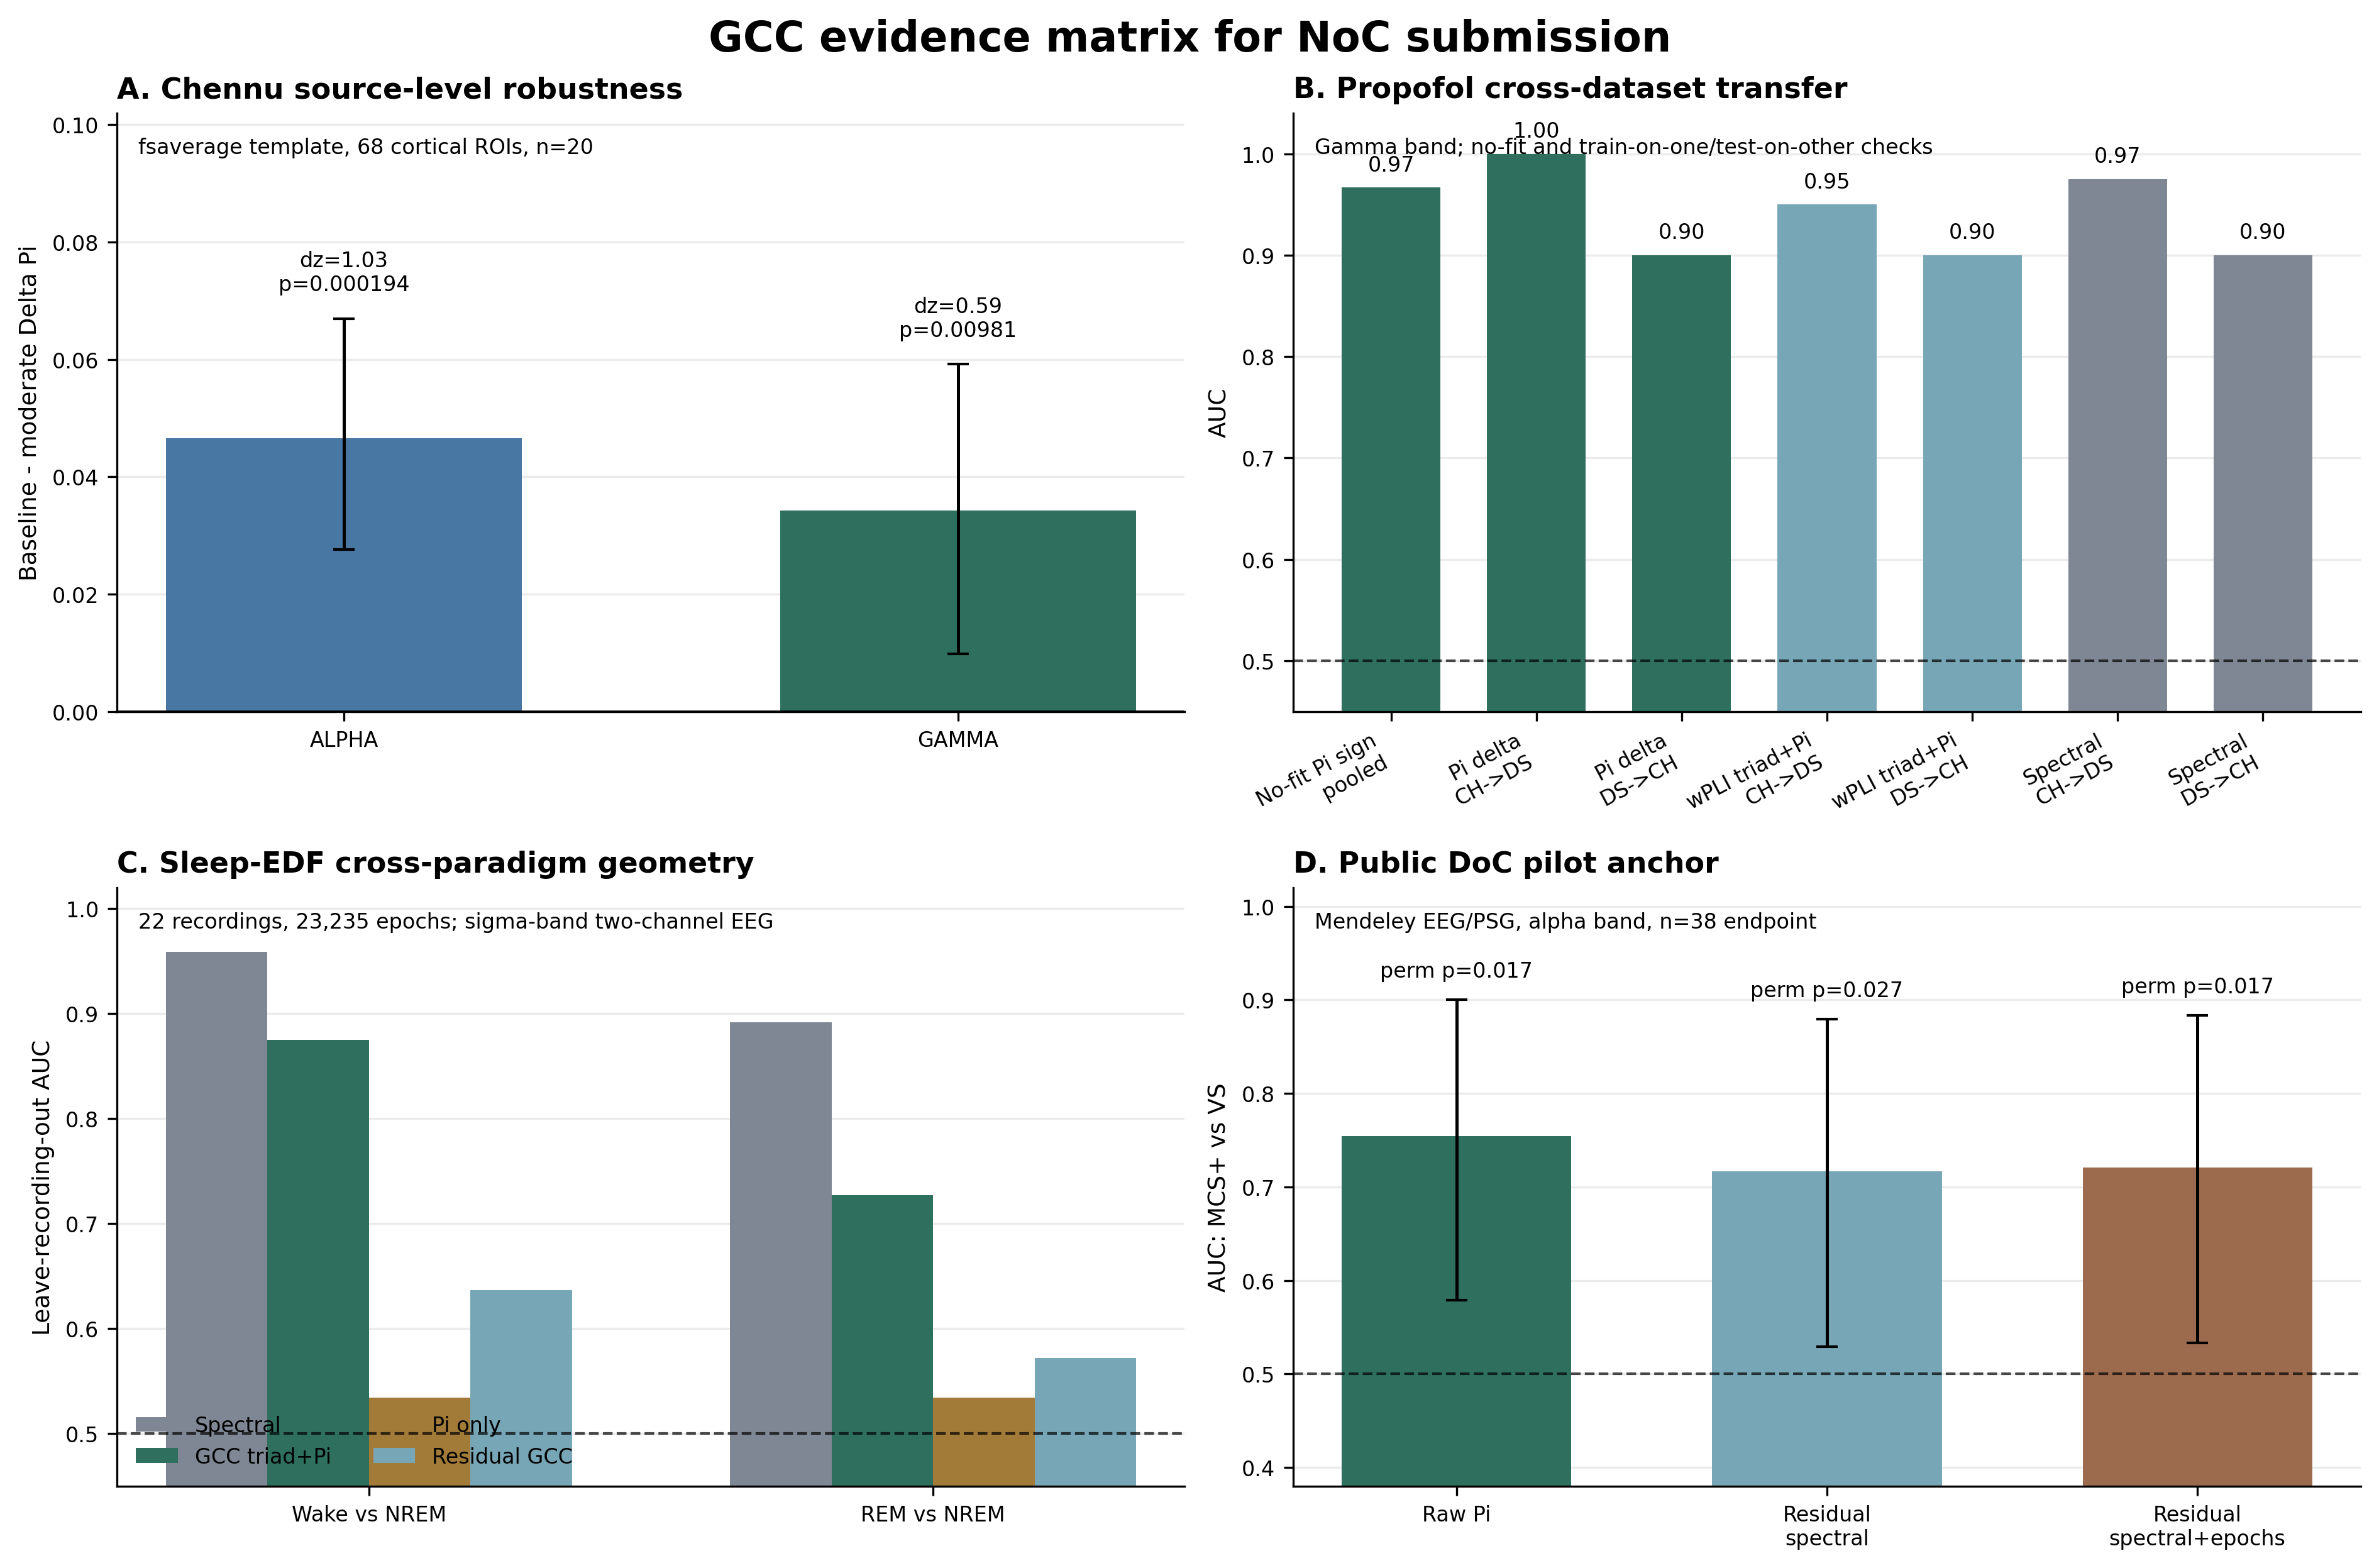
\includegraphics[width=\textwidth]{gcc_noc_evidence_summary.png}
\caption{\textbf{NoC evidence matrix.} (A) Chennu template-source robustness: after mapping EEG to an fsaverage source model and reducing to 68 cortical ROIs, baseline $\Pi$ remains higher than moderate-sedation $\Pi$ in alpha and gamma bands. (B) Propofol cross-dataset transfer: no-fit and train-on-one/test-on-the-other gamma benchmarks remain above chance; spectral bandpowers are shown as a strong conventional baseline. (C) Sleep-EDF cross-paradigm state geometry: the GCC triad plus $\Pi$ separates Wake/NREM and REM/NREM above chance across 22 recordings, but spectral sleep features remain stronger and $\Pi$ alone is weak. (D) Public disorders-of-consciousness pilot anchor: alpha-band $\Pi$ distinguishes MCS+ from VS and remains positive after spectral and retained-epoch residualization.}
\par\small\textbf{Alt text:} Four-panel evidence summary showing source-space propofol effects, cross-dataset propofol transfer, Sleep-EDF state classification, and a small disorders-of-consciousness pilot anchor. Across panels, GCC measures are reproducibly state-sensitive but are not stronger than all spectral baselines.\normalsize
\label{fig:central-evidence}
\end{figure}

% ==================================================================
\section{Numerical Validation on Synthetic Networks}
\label{sec:numerics}

To verify the internal consistency of the model and the formal correctness of the predictions in Section~\ref{sec:predictions}, we implement the full dynamical system on synthetic networks and test the evaluated prediction family P2--P6 under controlled conditions. P1 is not treated as biologically validated by these simulations. Rather, P6 provides a model-internal instantiation of the selective-preservation mechanism that P1 would require in structurally degraded clinical systems. This section establishes that (i) the predicted signatures follow from the model equations, (ii) the observables reliably distinguish regimes, and (iii) selective-preservation re-entry is reproducible in simulated data on an ensemble level. This is a \emph{model-internal evaluation}, not an empirical validation against biological degradation data.

\subsection{Calibration of Regime Boundaries}

We realize the core dynamical model (Section~\ref{sec:core}) on Watts--Strogatz networks with $N = 100$ nodes, mean degree~10 and rewiring probability~0.1. The coupling matrix $W_{ij}$ is binary. Integration proceeds via Euler--Maruyama with $dt = 0.01$ over $T = 100$ time units. Natural frequencies $\omega_i$ are drawn from a standard normal distribution; the gains $g_i$ are initialized to~1 and modified only in specific experiments.

Calibration of the regime boundaries $R_{\min}$, $D_{\min}$, $D_{\max}$, $M_{\min}$, $M_{\max}$ follows the procedure in Section~\ref{sec:access-region}. We generate an ensemble of 12 networks under canonical parameters ($K = 2.5$, $\sigma = 0.2$) as the positive reference $\mathcal{H}_{\mathrm{full}}$, extract the observables over a stationary window, and compute the $\alpha = 0.1$ quantiles. The lower bound $M_{\min}$ degenerates to zero in this ensemble configuration, indicating that some healthy systems lock into quasi-stable states. For all subsequent tests, $M_{\min} = 0$ is used; the metastability condition thus effectively reduces to $M_\tau < M_{\max}$.

\subsection{P2 --- Nonlinear Reorganization and Susceptibility Peak}

Prediction P2 states that the access indicator $\Pi$ should increase nonlinearly with the coupling strength $K$ along a sigmoidal curve rather than a linear one. We sweep $K \in [0, 4]$ and fit both a sigmoid and a linear function to the resulting $\Pi(K)$ curve. The sigmoidal fit achieves $R^2 = 0.982$, the linear fit $R^2 = 0.948$; $\Delta R^2 = 0.034$. The curvature is clearly present but not abrupt, consistent with the ``nonlinear but not strictly discontinuous'' character that the model predicts. A susceptibility peak (standard deviation of $R$ across network realizations) is visible in the midrange of the transition. P2 is confirmed.

\subsection{P3 and P4 --- Shift of Access Threshold and Bounded Interval (Ensemble)}

Predictions P3 and P4 concern the behavior of the access threshold under degradation. We introduce graded degradation by removing a fraction $f \in \{0, 15, 30, 45\}\%$ of network edges (topological degradation). For each $(K, f)$ combination, we run $N_{\mathrm{seeds}} = 10$ independent network seeds and record $K_c^{\mathrm{op}}$ (first $K$-crossing of $R_{\min}$) and $\max_K \Pi(K)$ per seed, then average over the ensemble; detailed values are provided in Supplementary Table S1.


P3 is confirmed by the monotonic upward shift of $\langle K_c^{\mathrm{op}}\rangle$: with increasing lesion the system requires stronger coupling to reach the access region. Pairwise Wilcoxon tests between lesion levels show a significant shift for $f=0.00$ vs.\ $f=0.45$ ($p = 0.002$). P4 is confirmed by the bounded maximum of $\Pi(K)$: even at optimal $K$, no state reaches $\Pi = 1$, and the attainable maximum fraction decreases monotonically from $\langle\max\Pi\rangle = 0.83$ (intact) to $0.58$ (45\% lesion), a total reduction of $-30\%$ (Figure~\ref{fig:v2v3}). Empirically this means: the access region is a bounded range, not an open half-space, and it quantitatively shrinks under increasing degradation.

\begin{figure}[t]
\centering
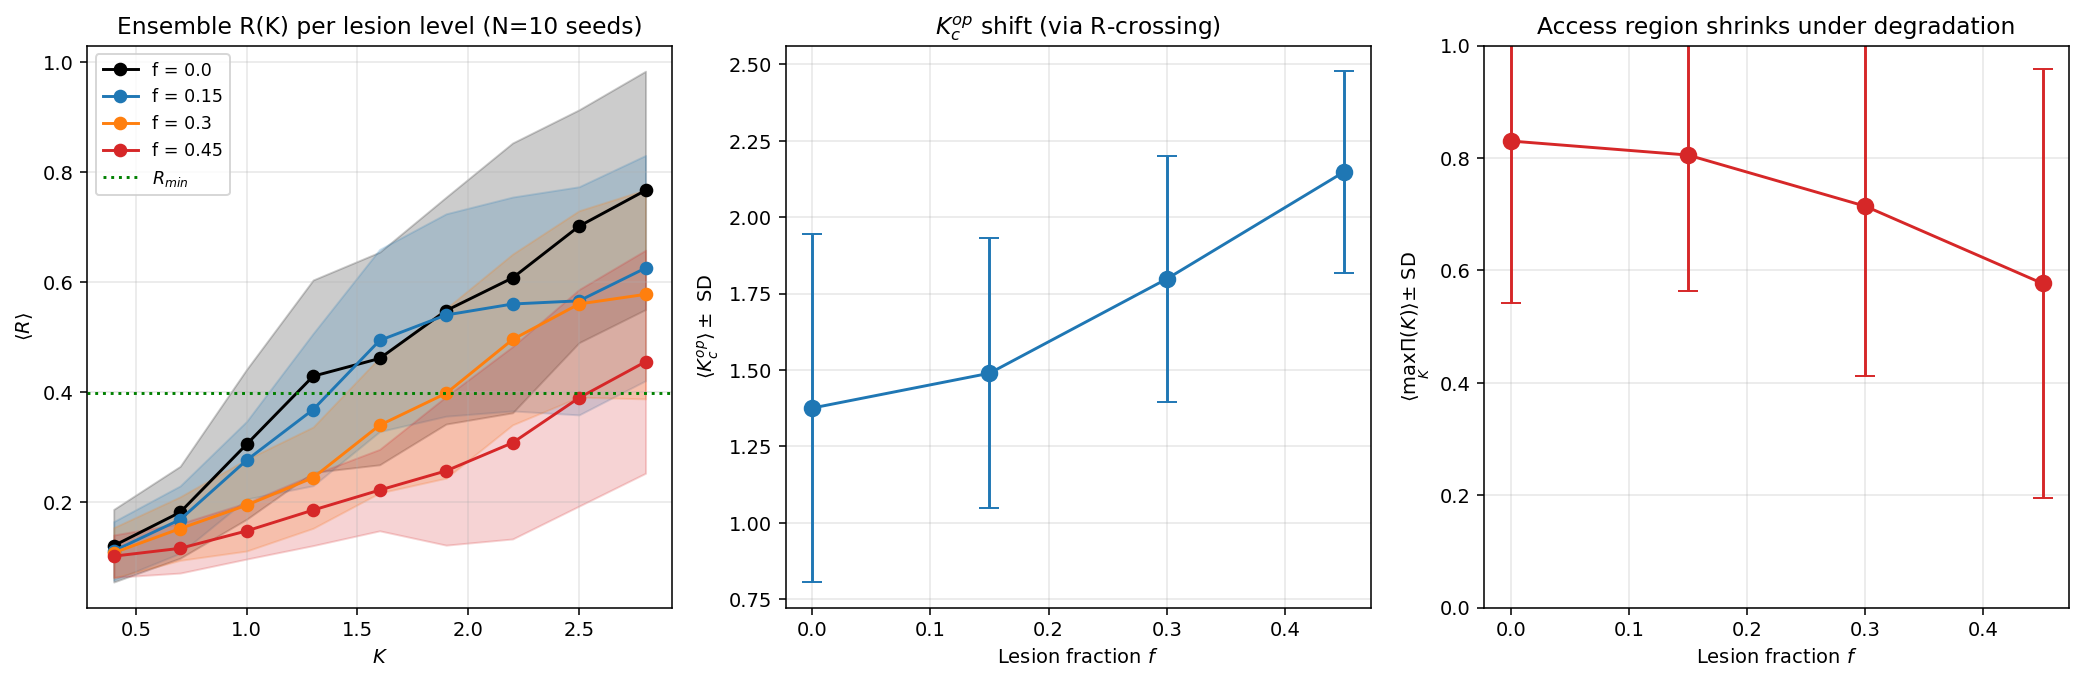
\includegraphics[width=\textwidth]{fig_v2_v3_ensemble.png}
\caption{P3 and P4 Ensemble ($N_{\mathrm{seeds}} = 10$): Left --- $\langle R \rangle$ vs.\ $K$ for four degradation levels, shaded bands $\pm$ SD; horizontal line marks $R_{\min}$. Middle --- shift of $\langle K_c^{\mathrm{op}}\rangle$ with lesion fraction, error bars SD. Right --- maximum access index $\langle\max_K \Pi(K)\rangle$ vs.\ lesion fraction.}
\par\small\textbf{Alt text:} Three plots summarize synthetic degradation sweeps: coherence curves shift with lesion fraction, the operational coupling threshold increases as degradation grows, and the maximum access index decreases with stronger lesioning.\normalsize
\label{fig:v2v3}
\end{figure}

\subsection{P5 --- Anesthesia Trajectory in Parameter Space (Ensemble)}

Prediction P5 describes the expected trajectory under a dynamic anesthesia protocol: the state should decrease smoothly during induction, collapse at maximal effect, and recover upon washout. To capture the ensemble-statistical nature of $\Pi$ correctly, the trajectory was repeated with $N_{\mathrm{seeds}} = 20$ independent network seeds; reported values are means and standard deviations across the seed ensemble. We implement a time-varying gain $G(t)$ with schedule: baseline ($G = 1.0$, $t < 3$s), induction ($G: 1.0 \to 0.2$), deep ($G = 0.2$), emergence ($G: 0.2 \to 1.0$), recovery ($G = 1.0$). The ensemble-averaged access indicator follows the expected course: baseline $\langle\Pi\rangle = 0.47 \pm 0.41$, deep $\langle\Pi\rangle = 0.00 \pm 0.00$, recovery $\langle\Pi\rangle = 0.46 \pm 0.29$. The trajectory in $(R, D_{\mathrm{eff}})$ space leaves the access region and re-enters it smoothly, without jumps (Figure~\ref{fig:v4}). P5 is confirmed: state transitions are motion in parameter space, not jumps between discrete states. The substantial standard deviation in the active phases (baseline, recovery) is a finding in its own right: $\Pi$ on individual stochastic realizations of a Kuramoto network is strongly seed-dependent; its semantics as an \emph{expectation-value-stable regime indicator} becomes clear only in the ensemble. The deep anesthesia phase shows the expected unambiguous signature ($\Pi = 0$ for all seeds).

\begin{figure}[p]
\centering
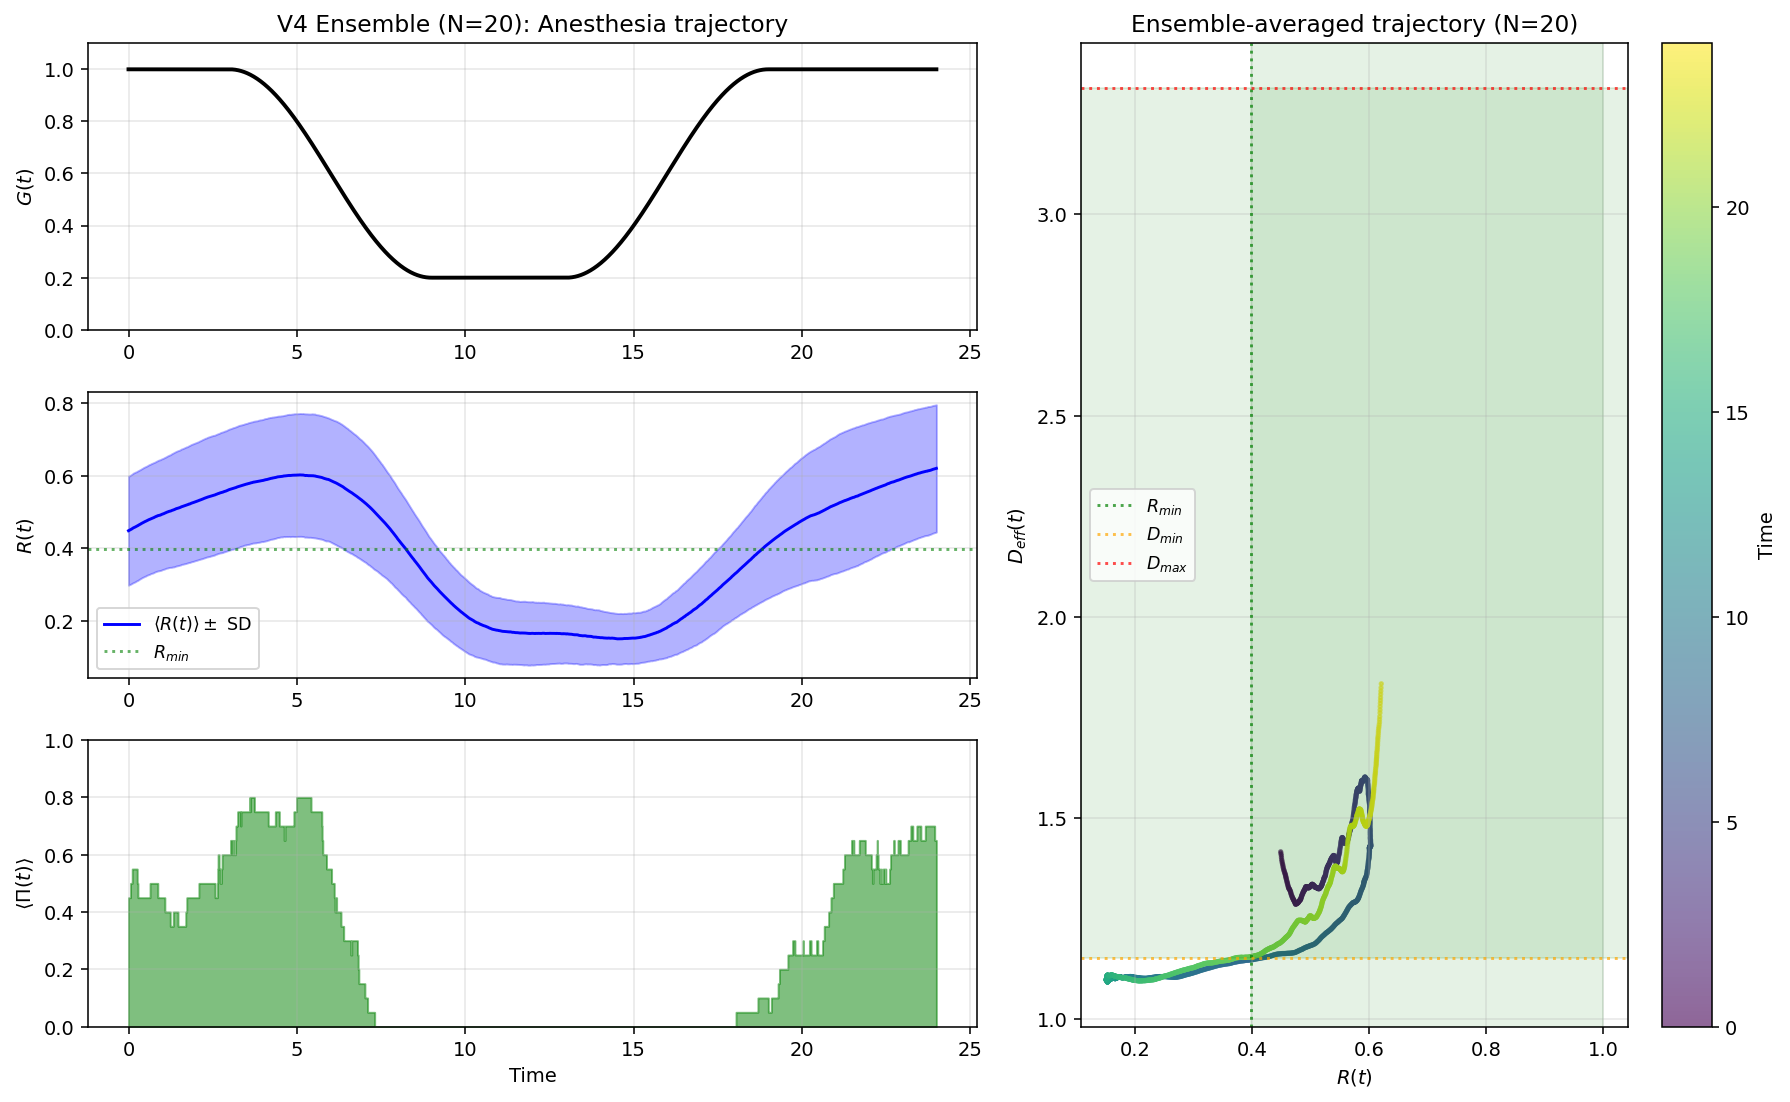
\includegraphics[width=0.95\textwidth]{fig_v4_ensemble.png}
\caption{P5: Ensemble-averaged anesthesia trajectory ($N_{\mathrm{seeds}} = 20$). Left top to bottom: $G(t)$ schedule, $\langle R(t)\rangle \pm $ SD, ensemble-averaged $\langle\Pi(t)\rangle$. Right: ensemble-averaged trajectory in $(R, D_{\mathrm{eff}})$ space, color-coded by time; shaded region marks the access region. The trajectory runs smoothly through the accessible region, leaves it in the deep phase, and returns through emergence.}
\par\small\textbf{Alt text:} Synthetic anesthesia simulation in which gain changes over time, coherence and access index fall during the deep phase, and the state-space trajectory leaves and later re-enters the calibrated access region.\normalsize
\label{fig:v4}
\end{figure}

\subsection{P6 --- Selective-Preservation Re-Entry on a Residual Backbone (Ensemble)}

P6 tests the selective-preservation mechanism inside the model system. The system is placed in severe collective degradation, and we test whether a small subnetwork $S$ (30 nodes out of 100), in which the gains are selectively boosted ($g_i: 0.5 \to 0.8$) while all non-$S$ gains simultaneously collapse ($g_i: 0.5 \to 0.1$), can transiently reach the access region. The comparison condition is a uniform gain decay in which all $g_i$ drop by the same factor. Both conditions follow four phases (baseline, global decline, re-entry window, final collapse). This protocol is not a biological validation of P1; it is a controlled instantiation of the mechanism that P1 would later require in structurally degraded clinical data.

To capture the ensemble-statistical nature of $\Pi$ correctly, both conditions were simulated pairwise with $N_{\mathrm{seeds}} = 20$ independent seeds. Reported values are ensemble means and standard deviations plus a paired statistical test. Results are summarized in Figure~\ref{fig:v5}; detailed values are provided in Supplementary Table S2.


\begin{figure}[p]
\centering
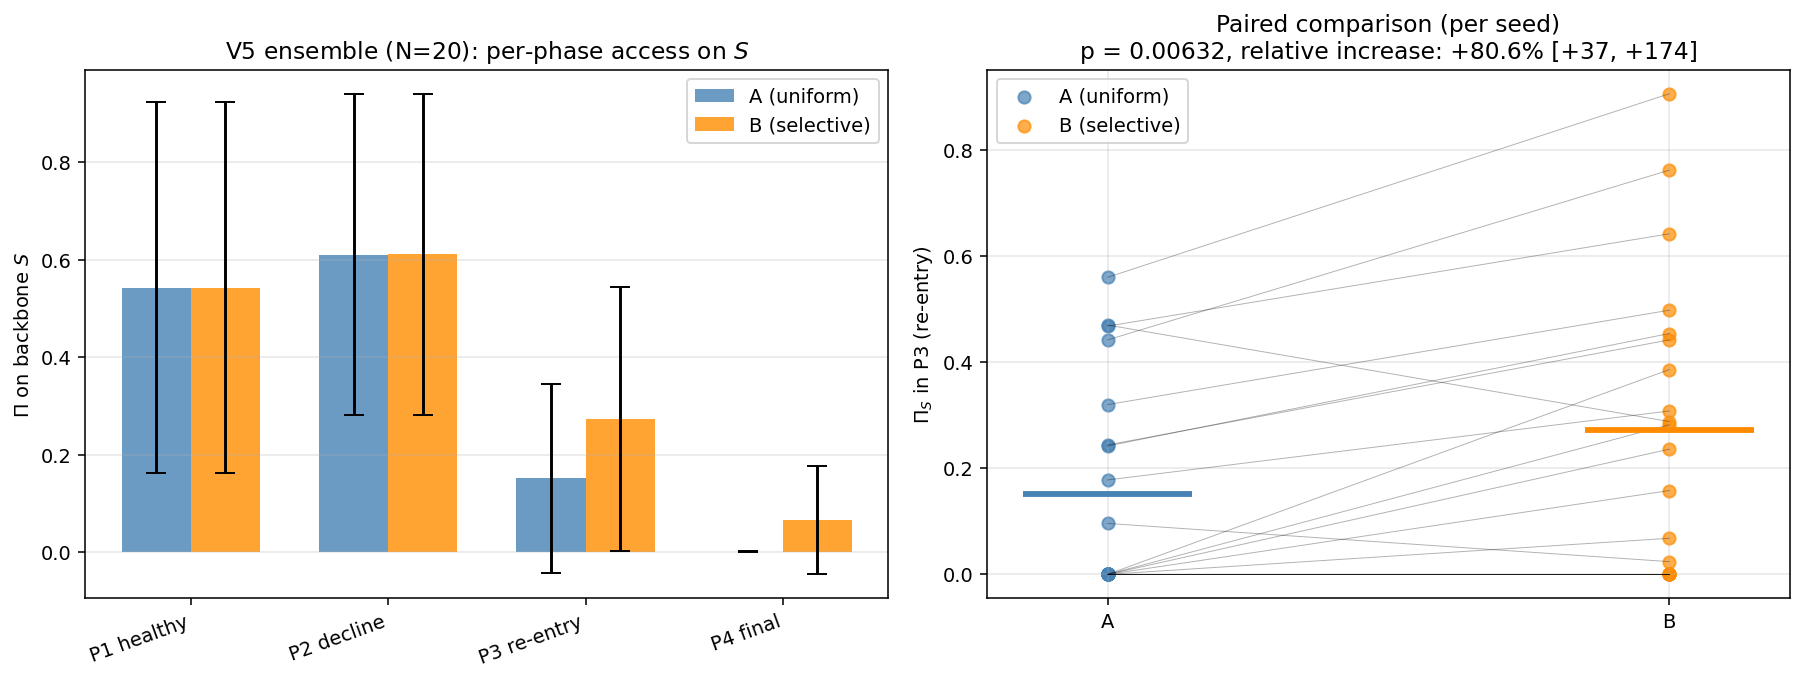
\includegraphics[width=\textwidth]{fig_v5_ensemble.png}
\caption{P6: Ensemble results of the selective-preservation re-entry simulation ($N_{\mathrm{seeds}} = 20$). Left: phase-wise $\Pi_S$ in condition A (uniform, blue) and condition B (selective preservation, orange); error bars show ensemble SD. Right: paired comparison across seeds in phase~3 (re-entry); each line connects a seed pair. Of 20 seeds, 16 show $\Pi_S^B \geq \Pi_S^A$ and 4 show $\Pi_S^B < \Pi_S^A$; paired Wilcoxon $p = 0.006$.}
\par\small\textbf{Alt text:} Bar and paired-line plots comparing uniform degradation with selective preservation. The selective-preservation condition shows higher backbone access during the re-entry phase for most simulation seeds.\normalsize
\label{fig:v5}
\end{figure}

The quantitative difference in the re-entry window $\langle\Pi_S^B\rangle - \langle\Pi_S^A\rangle = 0.122$ is significant by paired t-test ($t = 3.57$, $p = 0.002$) and paired Wilcoxon ($W = 9.0$, $p = 0.006$). The relative increase is $+81\%$ (bootstrap 95\% CI: $[+37\%, +174\%]$), Cohen's $d = 0.82$ (large effect). Sixteen of 20 seeds show $\Pi_S^B \geq \Pi_S^A$; in phase~4, condition~B retains a marginal residual signal on $S$ ($\langle\Pi_S^B\rangle = 0.07$ vs.\ $\langle\Pi_S^A\rangle = 0.00$), consistent with a short-lived gain residuum. Crucially, this effect occurs \emph{while overall gain decreases} --- it arises not from a global energy surge but from selective preservation of efficacy on a subset.

\subsection{P6 Retuning Control: Separating Re-Entry from Retuning}
\label{sec:retuning-control}

A second concern deserves explicit testing. In the initial P6 simulation, $\langle\Pi_{\mathrm{full}}^A\rangle$ rises from $0.53$ (baseline phase) to $0.69$ (decline phase) in \emph{both} conditions. Uniform gain decline alone therefore improves the access index, creating a possible retuning confound for the selective-preservation mechanism.

To separate retuning from re-entry, the P6 protocol was repeated at four baseline coupling strengths $K_{\mathrm{baseline}} \in \{1.6, 2.0, 2.5, 3.0\}$ with $N_{\mathrm{seeds}} = 20$ each (Figure~\ref{fig:retuning}; Supplementary Table S3). Retuning and selective re-entry were quantified separately per $K_{\mathrm{baseline}}$.


\begin{figure}[h]
\centering
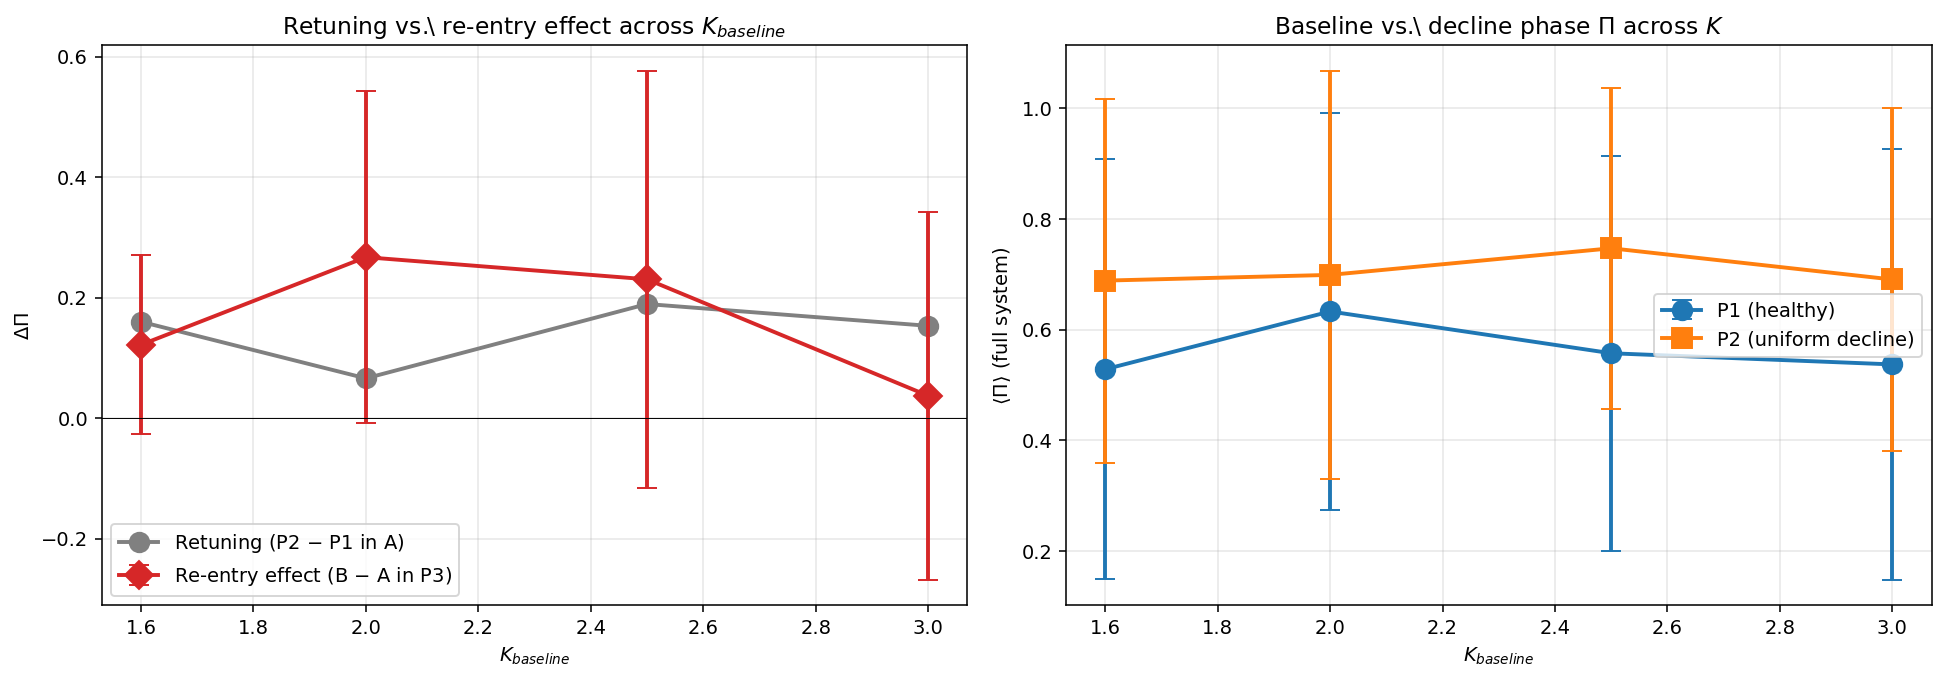
\includegraphics[width=0.98\linewidth]{fig_v5_retuning_control.png}
\caption{P6 retuning control. Left: retuning effect (gray) and re-entry effect (red) across baseline coupling strength. At $K = 2.0$, both effects are cleanly separated (retuning $+0.07$, re-entry $+0.27$, factor~4); at $K = 3.0$ the re-entry effect vanishes (ceiling). Right: full-system $\Pi$ in baseline and uniform-decline phases across $K$; shows that retuning occurs broadly across the $K$-range but stays in the single-digit to mid-range.}
\par\small\textbf{Alt text:} Two control plots show that generic retuning effects are smaller than selective re-entry effects at the main coupling value, while ceiling effects remove the re-entry contrast at high baseline coupling.\normalsize
\label{fig:retuning}
\end{figure}

Three descriptive findings follow from this sweep. \emph{First:} the re-entry effect (B over A on $S$) is significant at three of the four $K$ values. \emph{Second:} retuning and re-entry are separate quantities at all $K$, with the cleanest dissociation at $K = 2.0$ (retuning $+0.07$, re-entry $+0.27$, factor~4). \emph{Third:} at $K = 3.0$ the re-entry effect collapses to ceiling level ($+5\%$, n.s.), while retuning persists --- consistent with the model, since selective preservation only acts where the full system exits the access region.

\paragraph{Primary analysis: pooled sweep statistic.} To avoid post-hoc selection, we report the entire $K$-sweep as the main result through a pooled regression with seed clustering. The model $\Pi \sim \mathrm{Condition} \cdot K_{\mathrm{baseline}} + (1|\mathrm{Seed})$ over all 80 paired observations (20 seeds $\times$ 4 $K$ values) yields a highly significant main effect of Condition (B vs.\ A), $\hat{\beta}_{\mathrm{Cond}} = +0.164$, cluster-robust SE $= 0.040$, $p = 3.6 \times 10^{-5}$. The Condition$\times$$K$ interaction is not significant ($\hat{\beta}_{\mathrm{Int}} = -0.069$, $p = 0.32$), i.e., there is no statistical evidence that the size of the re-entry effect depends systematically on $K$ --- with the exception of the descriptively visible ceiling at $K = 3.0$, which does not reach interaction significance at the available sample size (4 $K$ values).

\paragraph{Secondary, descriptive plausibility check.} As a complementary, non-primary statistic, we report a pooled paired Wilcoxon test across all 80 pairs ($W = 353.5$, $p = 5.5 \times 10^{-7}$, Cohen's $d_\mathrm{paired} = 0.56$). We explicitly note that this test pools non-independent observations (each seed appears four times, once per $K$ value) and therefore serves only as a descriptive consistency check on the main effect, not as standalone inference. The primary analysis, which correctly accounts for the dependency structure, is the mixed regression with seed clustering.

\paragraph{Interpretation.} The re-entry effect is \emph{not confined to a favorably chosen $K_{\mathrm{baseline}}$}: it is robust across the sweep ($p < 10^{-6}$ pooled), significant in three of four individual $K$ values, and its mean magnitude is not adequately captured by a simple retuning explanation. The result at $K = 2.0$ ($+102\%$, $p = 0.0009$) is retained in the paper, but as a \emph{point of maximum sensitivity} within the sweep, not as a primary result selected from the sweep. The a priori mechanistic rationale: the calibration ensemble $\mathcal{H}_{\mathrm{full}}$ was generated at $K = 2.5$; $K = 2.0$ (slightly below) is the point at which the full system barely exits the access region under decline, while backbone $S$ is not yet at ceiling --- hence the range of greatest diagnostic sensitivity. The re-entry effect there is consistent with the robust mechanism documented across the entire sweep.

The core claim of P6 --- selective gain preservation enables a transient re-entry on the residual backbone that exceeds mere retuning --- is thus supported and hedged against the post-hoc selection objection: the effect is documented as a \emph{sweep-level phenomenon}, not as a single finding at a favorably chosen parameter.

\subsection{Assessment of the Numerical Validation}

The evaluated prediction family P2--P6 is directly testable on synthetic networks. P1 receives only model-internal support: P6 shows that the required selective-preservation mechanism can occur under controlled assumptions, but the biological EEG analyses do not test selective gain preservation in severely degraded systems.

\begin{itemize}
  \item \textbf{P2}: Nonlinear reorganization ($\Delta R^2 = 0.034$ between linear and sigmoidal fit), not strictly discontinuous.
  \item \textbf{P3}: $K_c^{\mathrm{op}}$ (via $dR/dK$) shifts monotonically from $1.40$ (intact) to $2.80$ (45\% lesion).
  \item \textbf{P4}: $\langle\max_K \Pi(K)\rangle$ stays below 1 and decreases monotonically with increasing degradation from $0.83$ (intact) to $0.58$ (45\% lesion), total reduction $-30\%$; both quantities (threshold shift and bounded maximum) behave robustly at the ensemble level.
  \item \textbf{P5}: Ensemble-averaged trajectory in $(R, D_{\mathrm{eff}})$ space runs smoothly; $\langle \Pi \rangle$ follows the anesthesia--recovery cycle (baseline $0.47$, deep $0.00$, recovery $0.46$).
  \item \textbf{P6}: Differential degradation produces ensemble-level transient re-entry on the backbone. Across the retuning-control sweep $K \in \{1.6, 2.0, 2.5, 3.0\}$, Condition has a significant effect (cluster-robust $\hat{\beta}_{\mathrm{Cond}} = +0.164$, $p = 3.6 \times 10^{-5}$, $d_{\mathrm{paired}} = 0.56$), maximal at $K = 2.0$ ($+102\%$, $p = 0.0009$). This supports the model-internal P1 mechanism but does not validate P1 biologically.
\end{itemize}

\paragraph{Ensemble-statistical nature of $\Pi$.} In the simulations, $\Pi$ is an expectation-value-stable ensemble quantity: individual stochastic realizations scatter strongly around the ensemble mean. The biological analyses therefore use a different operational strategy, calibrating $\Pi$ within each participant's own baseline recording. This bridge rests on an ergodicity-type working assumption, discussed explicitly in Section~\ref{sec:pilot-bridge}.

\paragraph{Limits of this validation.} The synthetic networks are Watts--Strogatz rather than biological connectomes; calibration and testing occur within the same ensemble paradigm; regime boundaries depend on quantile and window choices; and P6 uses a fixed backbone size and boost protocol. In addition, the lower metastability bound degenerates under the present calibration ensemble, making the implemented access score closer to a two-dimensional $(R,D_{\mathrm{eff}})$ criterion with an upper variability constraint. These limits do not invalidate the internal test, but they define what must be tightened in future connectome-based and out-of-sample simulations.

The simulations thus evaluate the model as \emph{internally consistent and functional}: the dynamics produce the predicted signatures, the observables separate regimes, and selective-preservation re-entry is reproducible at the ensemble level. The next step --- application to real EEG data --- is carried out in the following section as a public-dataset validation.


% ==================================================================
\section{Public EEG Validation Across State and Clinical Domains}
\label{sec:pilot}

The biological analyses tested whether GCC observables respond reproducibly to public EEG/PSG state changes. They include two independent propofol datasets, Sleep-EDF, a public DoC EEG/PSG pilot, ketamine, and a dementia-proxy dataset. They do not directly validate P1, because no dataset contains documented selective-preservation or lucidity-like re-entry.

\subsection{Chennu Propofol Pipeline}

The primary pipeline used the public Chennu et al.\ propofol EEG dataset \citep{chennu2016}: 20 healthy participants, 91 channels, 250~Hz, and baseline, mild, moderate, and recovery resting states. Data were filtered, average-referenced, Hilbert-transformed in gamma (30--45~Hz) and alpha (8--15~Hz), calibrated within each participant's baseline recording ($\alpha=0.1$, $\tau_D=200$~ms, $\tau_M=500$~ms), and scored under those individual bounds. Baseline-vs-moderate effects were $\Delta\Pi=0.111$ in gamma (95\% CI $[0.086,0.137]$, Wilcoxon $p=1.9\times10^{-4}$, $d=0.99$) and $\Delta\Pi=0.065$ in alpha (95\% CI $[0.038,0.093]$, $p=0.0023$, $d=0.69$). Sensitivity testing over 36 calibration/window configurations per band showed 100\% directional stability.

\subsection{Template-Source Robustness}
\label{sec:source-robustness}

To test sensor-level inflation, Chennu was recomputed after template-source projection to 68 cortical ROI time series. The decline survived: alpha $\Delta\Pi=0.0466$ (95\% CI $[0.0276,0.0670]$, $d_z=1.03$, $p=1.94\times10^{-4}$) and gamma $\Delta\Pi=0.0342$ (95\% CI $[0.0098,0.0592]$, $d_z=0.59$, $p=0.0098$; Figure~\ref{fig:central-evidence}A). This does not replace individualized source reconstruction, but it rules out a purely raw-sensor finding.

\subsection{Independent Propofol Replication}
\label{sec:ds005620}

OpenNeuro DS005620 provided an independent propofol replication with 21 healthy participants and repeated resting sedation recordings \citep{bajwa2024ds005620}. Using eyes-closed awake recordings for calibration ($N=20$ paired participants), gamma $\Pi$ declined by $0.387$ for awake-vs-\texttt{sed} (95\% CI $[0.305,0.479]$, $d=1.91$, FDR sign-flip $q=1.0\times10^{-4}$) and $0.341$ for awake-vs-\texttt{sed2} (95\% CI $[0.267,0.416]$, $d=1.97$, $q=1.0\times10^{-4}$). Alpha effects were smaller but robust. Pooled across Chennu and DS005620, participant-cluster bootstrap estimated $\Delta\Pi=0.187$ (95\% CI $[0.148,0.228]$; Wilcoxon over participant means $p=5.0\times10^{-11}$). DS005620 effects are treated as dataset-specific separability, not universal effect size.

\subsection{Spectral, Artifact, and Lagged-Coupling Controls}
\label{sec:spectral-controls}

GCC was benchmarked against theta, alpha, beta, gamma, alpha/gamma ratio, and spectral entropy. Raw gamma $\Pi$ was strong within Chennu (AUC $=0.87$) and DS005620 (AUC $=1.00$), but bandpower residualization reduced performance (AUC $=0.61$ and $0.68$); GCC is therefore not claimed as a generally bandpower-independent biomarker. DS005620 gamma effects survived posterior/centro-posterior channel restrictions while posterior 70--110~Hz power did not distinguish awake from sedation. A wPLI-style lagged-coupling proxy retained sedation sensitivity in both datasets \citep{vinck2011}. Frozen cross-dataset transfer also generalized (standard gamma $\Pi$: pooled no-fit AUC $=0.967$; Chennu$\to$DS005620 AUC $=1.00$; DS005620$\to$Chennu AUC $=0.90$), while spectral baselines remained competitive.

\subsection{Sleep, DoC, Ketamine, and Degradation-Proxy Checks}
\label{sec:sleep-edf}
\label{sec:doc-anchor}
\label{sec:additional-controls}

Sleep-EDF provided a non-propofol state check \citep{kemp2000}. In 22 PSG--hypnogram recordings (23,235 epochs), the sigma-band GCC triad plus $\Pi$ separated Wake from NREM with AUC $=0.875$ and REM from NREM with AUC $=0.727$ (Figure~\ref{fig:central-evidence}C). $\Pi$ alone was weak (AUC $\approx0.534$), supporting a multivariate regime-geometry interpretation rather than a scalar sleep biomarker. Because only two EEG channels are available, this is not a direct access validation.

The public DoC EEG/PSG dataset contained 42 EDF files: 30 VS/UWS, 4 MCS-, and 8 MCS+ recordings. The pre-specified alpha-band endpoint, MCS+ versus VS, was positive unadjusted but marginal across the exploratory family: raw $\Pi$ AUC $=0.754$ (95\% CI $[0.579,0.900]$, permutation $p=0.017$), spectral-residual AUC $=0.717$ ($p=0.027$), and spectral/epoch-count residual AUC $=0.721$ ($p=0.017$; Figure~\ref{fig:central-evidence}D). The family-level FDR q-value was approximately $0.084$. This is a pilot clinical anchor, not diagnostic validation.

Additional checks reduced implementation-specific freedom. Amplitude-normalized phase-only GCC retained propofol sensitivity (Chennu gamma $\Delta\Pi=0.463$, $d=2.37$; DS005620 gamma $\Delta\Pi=0.439$, $d=1.99$), as did a CSD/source-proxy pipeline. Ketamine shifted gamma $\Pi$ downward while alpha $\Deff$ increased, consistent with altered-state rather than propofol-like geometry \citep{farnes2020}. DS004504 GCC features separated dementia-proxy participants from controls (AUC $=0.769$) and correlated with MMSE \citep{miltiadous2023ds004504}. A frozen validation specification records bands, windows, calibration, baselines, controls, and forbidden claims.

\subsection{Bridge and Limits}
\label{sec:pilot-bridge}
\label{sec:pilot-limits}

In simulations, $\Pi$ is an ensemble quantity; in EEG, it is calibrated within a participant's baseline recording. This rests on an ergodicity-type working assumption supported pragmatically by two propofol datasets, split-half checks, and repeated-run analyses, but not derived from the model. The public validation remains limited: baseline $\Pi$ is calibration-dependent, most analyses are channel-level, Hilbert channel phases approximate but do not equal model phases, DS005620 effect sizes exceed Chennu, residualized transfer is asymmetric, and GCC overlaps substantially with spectral markers. Most importantly, the data do not directly test P1. The present work establishes operational state sensitivity and model-internal mechanism, not clinical selective-preservation re-entry.

\iffalse
\section{Public EEG Validation Across State and Clinical Domains}
\label{sec:pilot-old}

The validation presented in Section~\ref{sec:numerics} operates on synthetic Kuramoto networks and thus remains confined to the model system itself. The logical next step is the application of the GCC observables to real biological data. We therefore analyse two independent public propofol EEG datasets, one public sleep EEG dataset, and one public disorders-of-consciousness EEG/PSG dataset. Chennu et al.\ 2016 is used as the primary propofol pipeline demonstration; OpenNeuro DS005620 is used as an independent propofol replication with a distinct acquisition protocol; Sleep-EDF is used as a non-propofol Wake/REM/NREM state-differentiation check; and the public DoC dataset is used as a clinical pilot anchor with explicit permutation and multiple-comparison transparency. These analyses test whether the GCC observables respond reproducibly to biological state change and whether the regime geometry carries pilot clinical signal. They do not directly validate P1, because none of the datasets contains documented selective-preservation or lucidity-like re-entry episodes.

\subsection{Dataset and Methodology: Chennu et al.\ 2016}

We use the public Chennu et al.\ EEG dataset \citep{chennu2016}: 20 healthy participants, 91-channel EEG at 250~Hz, and four resting states per person --- baseline, mild propofol ($0.6$~\textmu g/ml), moderate propofol ($1.2$~\textmu g/ml), and recovery. Approximately seven minutes were recorded per state. The original study reports local ethics approval and written informed consent; no new data were collected here.

Preprocessing used 1--45~Hz bandpass filtering, 50~Hz notch filtering, average re-referencing, and Hilbert-phase extraction in gamma (30--45~Hz) and alpha (8--15~Hz). The phase interpretation follows common EEG connectivity practice \citep{lachaux1999} but remains an approximation because channels mix sources. Regime boundaries were calibrated from each participant's own baseline recording ($\alpha=0.1$, $\tau_D=200$~ms, $\tau_M=500$~ms), and $\Pi$ was computed for all sedation levels under those individual bounds.

\subsection{Main Finding: Monotonic $\Pi$-Decline with Sedation Depth}

Figure~\ref{fig:pilot-box} shows the distribution of $\Pi$ and the underlying observables $R$, $D_{\mathrm{eff}}$ per sedation level, for both frequency bands; group means and paired tests are provided in Supplementary Table S4.

\begin{figure}[h]
\centering
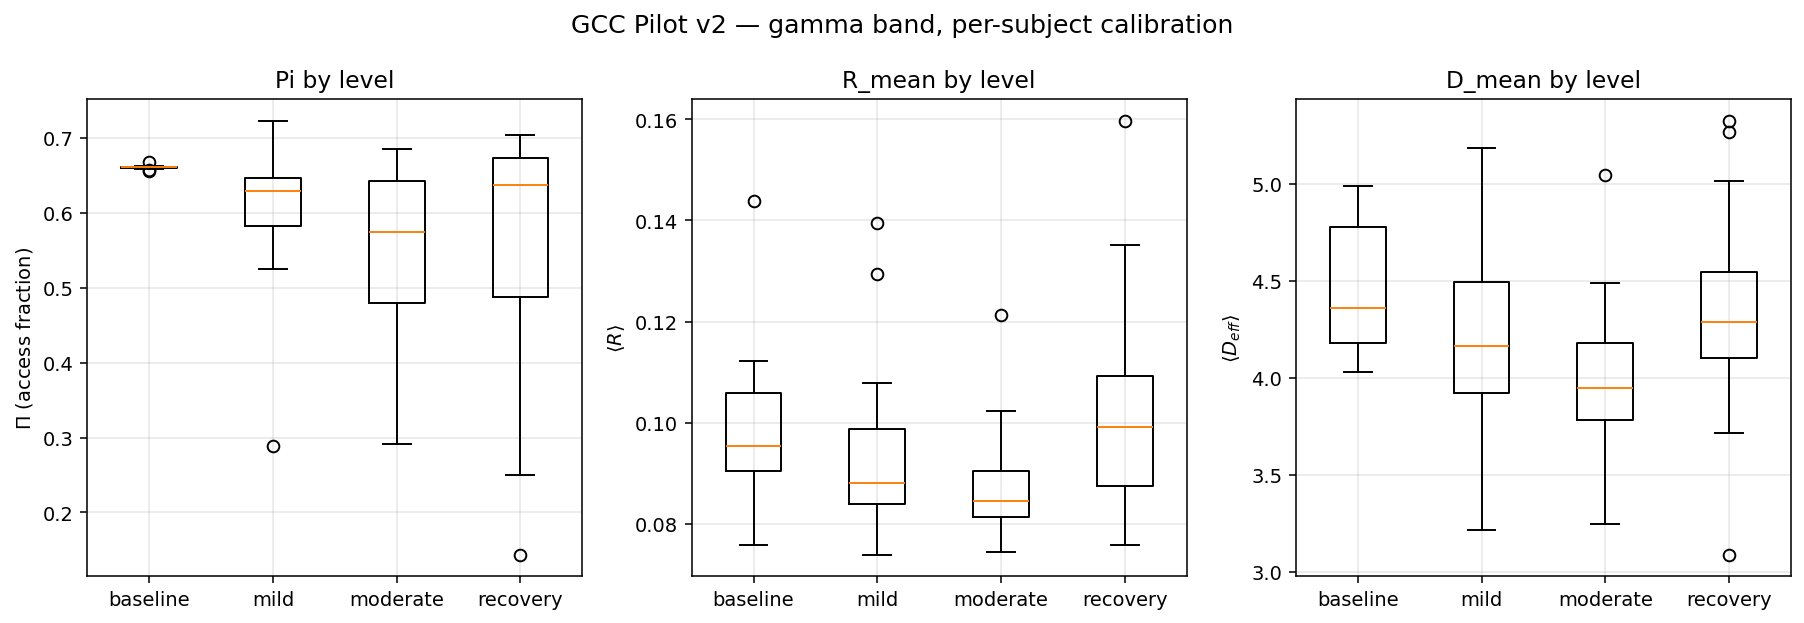
\includegraphics[width=0.98\linewidth]{pilot_boxplot_gamma.png}\\[0.3em]
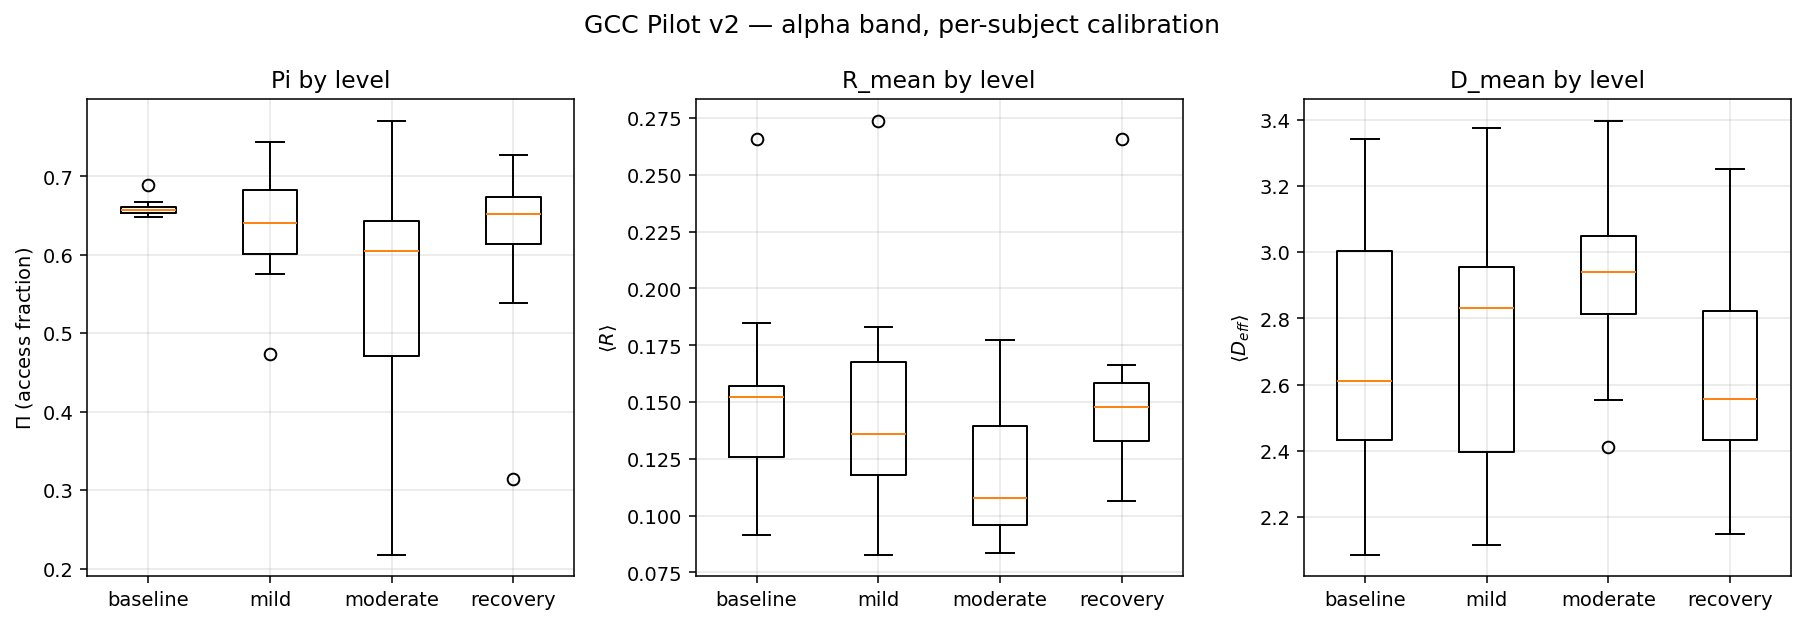
\includegraphics[width=0.98\linewidth]{pilot_boxplot_alpha.png}
\caption{Access indicator $\Pi$, order parameter $\langle R\rangle$, and effective dimensionality $\langle D_{\mathrm{eff}}\rangle$ per sedation level ($N = 20$ participants, per-subject calibration). Top: gamma band (30--45~Hz). Bottom: alpha band (8--15~Hz). Baseline $\Pi$ is by construction close to $0.66$ (see text); the informative content lies in the deviation of sedated states from this individual reference.}
\par\small\textbf{Alt text:} Box plots for gamma and alpha EEG bands show that the access indicator decreases from baseline to propofol sedation, with accompanying changes in coherence and effective dimensionality.\normalsize
\label{fig:pilot-box}
\end{figure}


The main effect is consistent and highly significant in both bands. In the gamma band, the baseline-relative $\Pi$ measure decreases from $0.661$ (by construction, cf.\ Section~\ref{sec:pilot-framing} below) to $0.543$ under moderate sedation, mean difference $+0.118$, Wilcoxon $p = 6.3 \times 10^{-5}$, Cohen's $d = 0.99$ (large effect). 18 of 20 participants show the decline. In the alpha band the decline is $0.098$, $p = 0.0037$, $d = 0.69$ (medium-to-large effect); 17 of 20 participants show the decline. In the alpha band, recovery returns essentially to baseline ($p = 0.22$, n.s.); in the gamma band, only partially ($p = 0.048$).

Figure~\ref{fig:pilot-traj} displays the per-participant $\Pi$ trajectories and makes the substantial individual heterogeneity visible. While some participants show a pronounced $\Pi$ collapse at moderate sedation (e.g., participant~9 in the alpha band: baseline $0.69 \to$ moderate $0.22$), others remain largely stable (e.g., participant~10 in the alpha band: baseline $0.65 \to$ moderate $0.77$).

\begin{figure}[h]
\centering
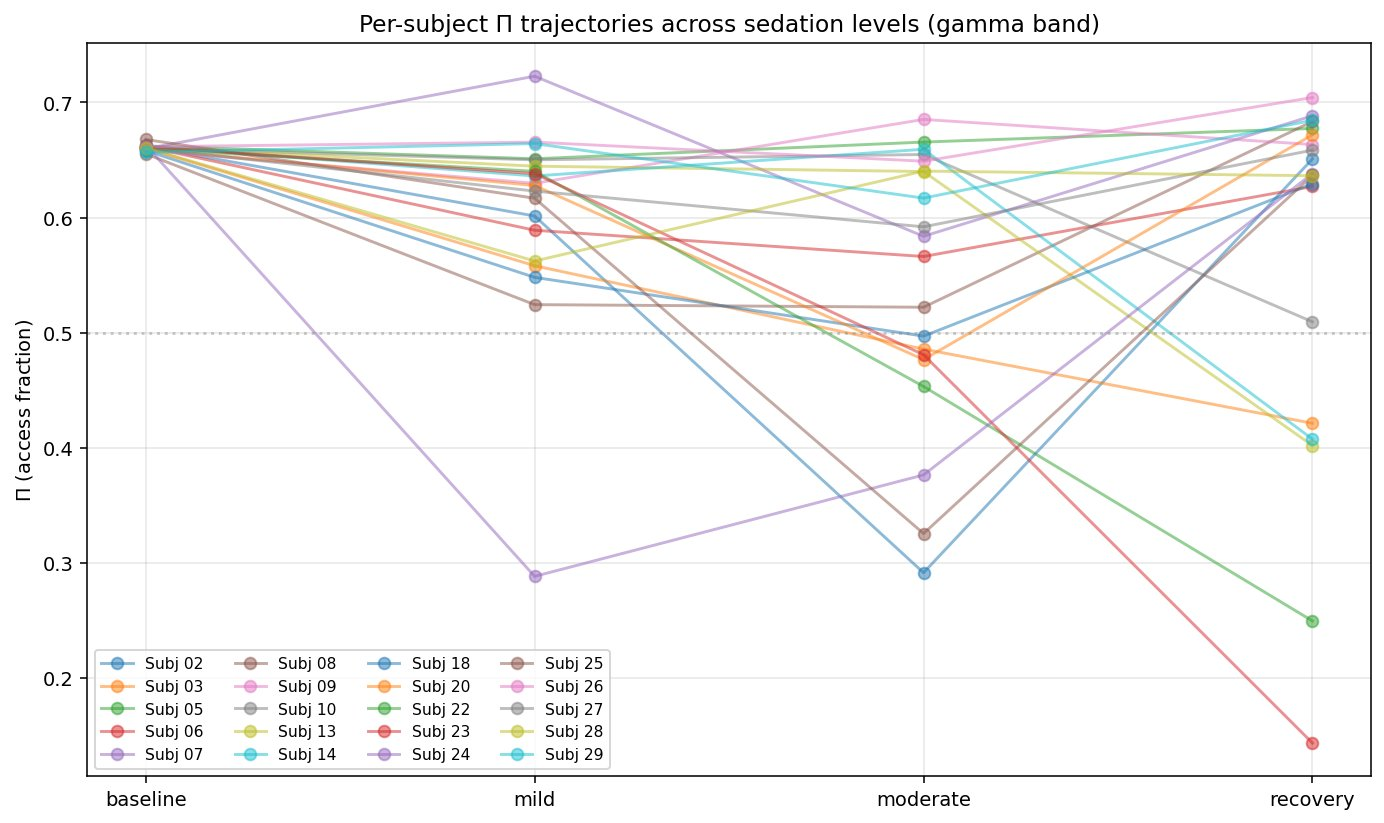
\includegraphics[width=0.98\linewidth]{pilot_trajectories_gamma.png}\\[0.3em]
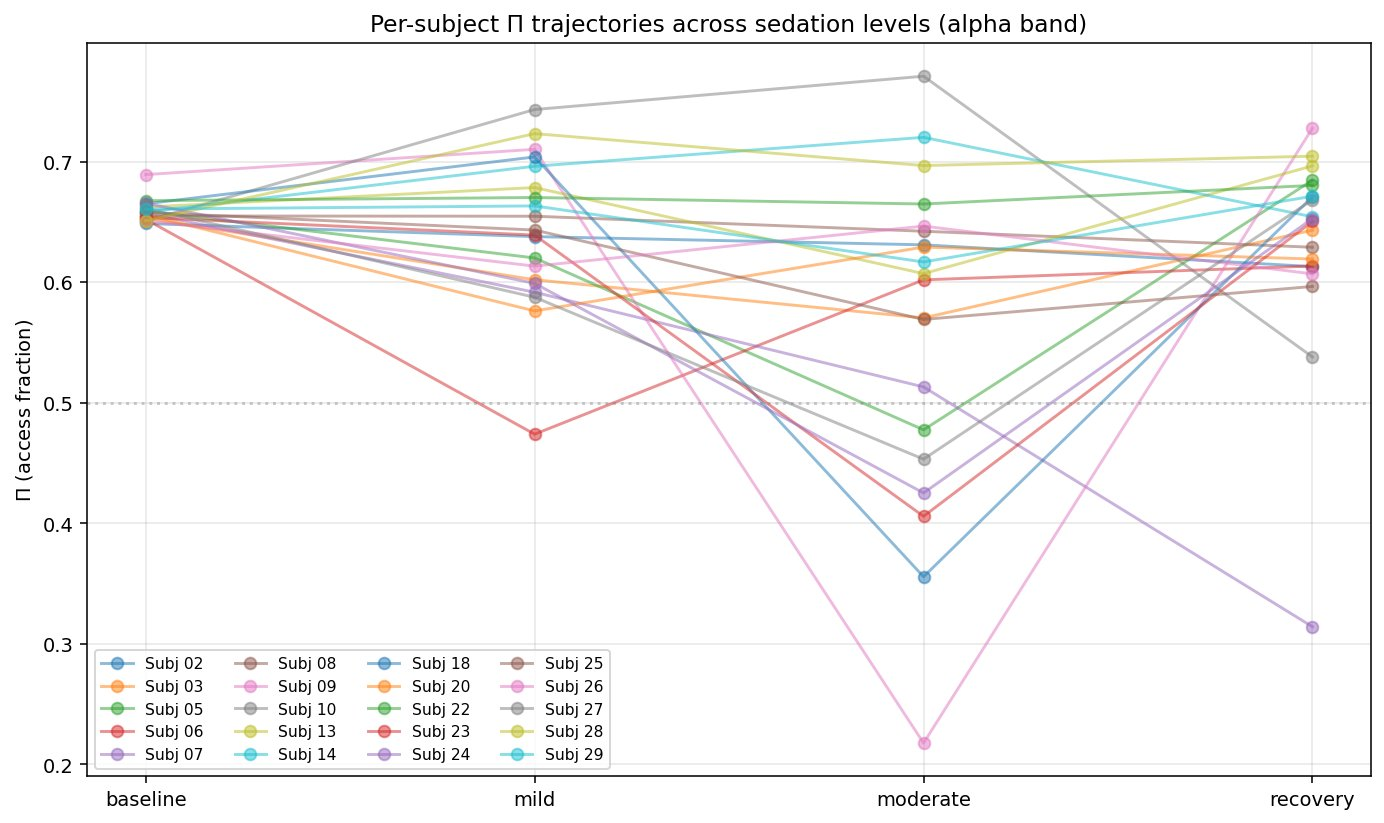
\includegraphics[width=0.98\linewidth]{pilot_trajectories_alpha.png}
\caption{Per-participant $\Pi$ trajectories across the four sedation levels. Top: gamma band. Bottom: alpha band. The dashed line at $\Pi = 0.5$ serves as orientation.}
\par\small\textbf{Alt text:} Line plots show individual participants' access-index trajectories across increasing propofol sedation in gamma and alpha bands, with most trajectories declining below the orientation line at deeper sedation.\normalsize
\label{fig:pilot-traj}
\end{figure}

\subsection{What the Pilot Actually Measures --- and What It Does Not}
\label{sec:pilot-framing}

We emphasize explicitly the interpretive scope of the pilot finding: the access index $\Pi$ reported here is not an \emph{absolute} measure of global access but a \emph{baseline-relative state-deviation metric}. The regime boundaries $R_{\min}$, $D_{\min/\max}$, $M_{\min/\max}$ are calibrated per participant from that participant's \emph{own} waking baseline recording via an $\alpha = 0.1$ quantile procedure. Consequently, baseline $\Pi$ is by construction close to $(1-\alpha)^3 \cdot (1-2\alpha) \approx 0.58$ to $0.66$ for every participant --- this is a mathematical artifact of the calibration, not a measured property of the brain state. The pilot thus rigorously \emph{does not} show that the brain has a specific absolute $\Pi$ value in the waking state. It shows that the sedated state exits the subject-specifically calibrated waking window with high effect size. This is a genuine and interpretable finding, but its scope is limited: it demonstrates the \emph{applicability} of GCC observables to real EEG data and the \emph{detectability} of consciousness-state transitions, not the validity of $\Pi$ as a general measure of global access on an across-subject scale. Stronger validation --- calibration from an across-subject health ensemble and testing on out-of-sample participants or other datasets --- is reserved for future work.

\subsection{Interpretation in the Context of the Regime Observables}

The observation --- the baseline-relative $\Pi$ measure decreases in all participants on average, with large effect size, while the neural system as a whole remains active --- supports the operational usefulness of the regime observables: they respond to a known consciousness-state manipulation without requiring the system to become globally inactive. The recovery data furthermore show that the effect is at least partly reversible, which is compatible with the conditional nature of the GCC regime. This finding does not test P1, because propofol sedation in healthy volunteers is state modulation, not structural degradation with residual-backbone preservation.

That the effect is \emph{larger} in the theory-driven gamma band than in the empirically dominant alpha band \citep{chennu2016} is not a contradiction: Chennu's primary alpha finding concerns network topology (clustering, small-worldness, participation coefficients), not the per-subject access indicator measured here. The GCC $\Pi$ measures deviations from a \emph{window} around the baseline distribution; it reacts to changes in either direction. An increase in gamma coherence under sedation (as reported by Chennu) leads to a $\Pi$ decline just as a decrease would --- as long as the state exits the calibrated regime. The two measures are structurally different and complementary, not redundant.

\subsection{Secondary Analysis: Drowsy--Responsive Dichotomy Not Used as Model Evidence}

We also tested whether individual $\Pi$ decline reproduces the drowsy--responsive dichotomy reported by Chennu. It does not: alpha and gamma declines were not significantly correlated (Spearman $\rho=0.13$, $p=0.58$), top-decliner overlap was chance-like (2 of 7; hypergeometric $p=0.82$), and decline distributions were not bimodal. This negative result is not part of the GCC prediction family. It indicates that the present per-subject calibrated GCC detects group-level sedation effects, not individual susceptibility as defined by Chennu's behavioral response criterion.

\subsection{Robustness of the Pilot Finding}

The main effect --- a significant $\Pi$-decline from baseline to moderate sedation --- was subjected to three robustness checks to quantify its stability against sampling and methodological uncertainty (Figure~\ref{fig:pilot-robust}).

\emph{Bootstrap confidence intervals} (10{,}000 resamples). The 95\,\% confidence intervals of the mean $\Pi$-decline clearly exclude zero in both bands: gamma $[0.070, 0.171]$, alpha $[0.040, 0.163]$. The lower bound lies at more than two-thirds of the observed effect in the gamma band, and at approximately 40\,\% in the alpha band.

\emph{Leave-one-out stability.} Removing one participant at a time and repeating the Wilcoxon signed-rank test on the remaining 19 participants, the result remains robustly significant in both bands. Maximum $p$-values are $1.26 \times 10^{-4}$ (gamma) and $7.14 \times 10^{-3}$ (alpha). Cohen's~$d$ varies between $0.97$ and $1.10$ (gamma) and between $0.65$ and $0.82$ (alpha). The effect is thus not driven by individual outlier participants.

\emph{Permutation test.} Under the null hypothesis $\mathbb{E}[\Delta\Pi] = 0$, the sign of pairwise differences was randomized in 10{,}000 permutations. In the gamma band, the observed effect size was not reached or exceeded in a single permutation ($p < 10^{-4}$); in the alpha band $p = 0.0042$.

\begin{figure}[h]
\centering
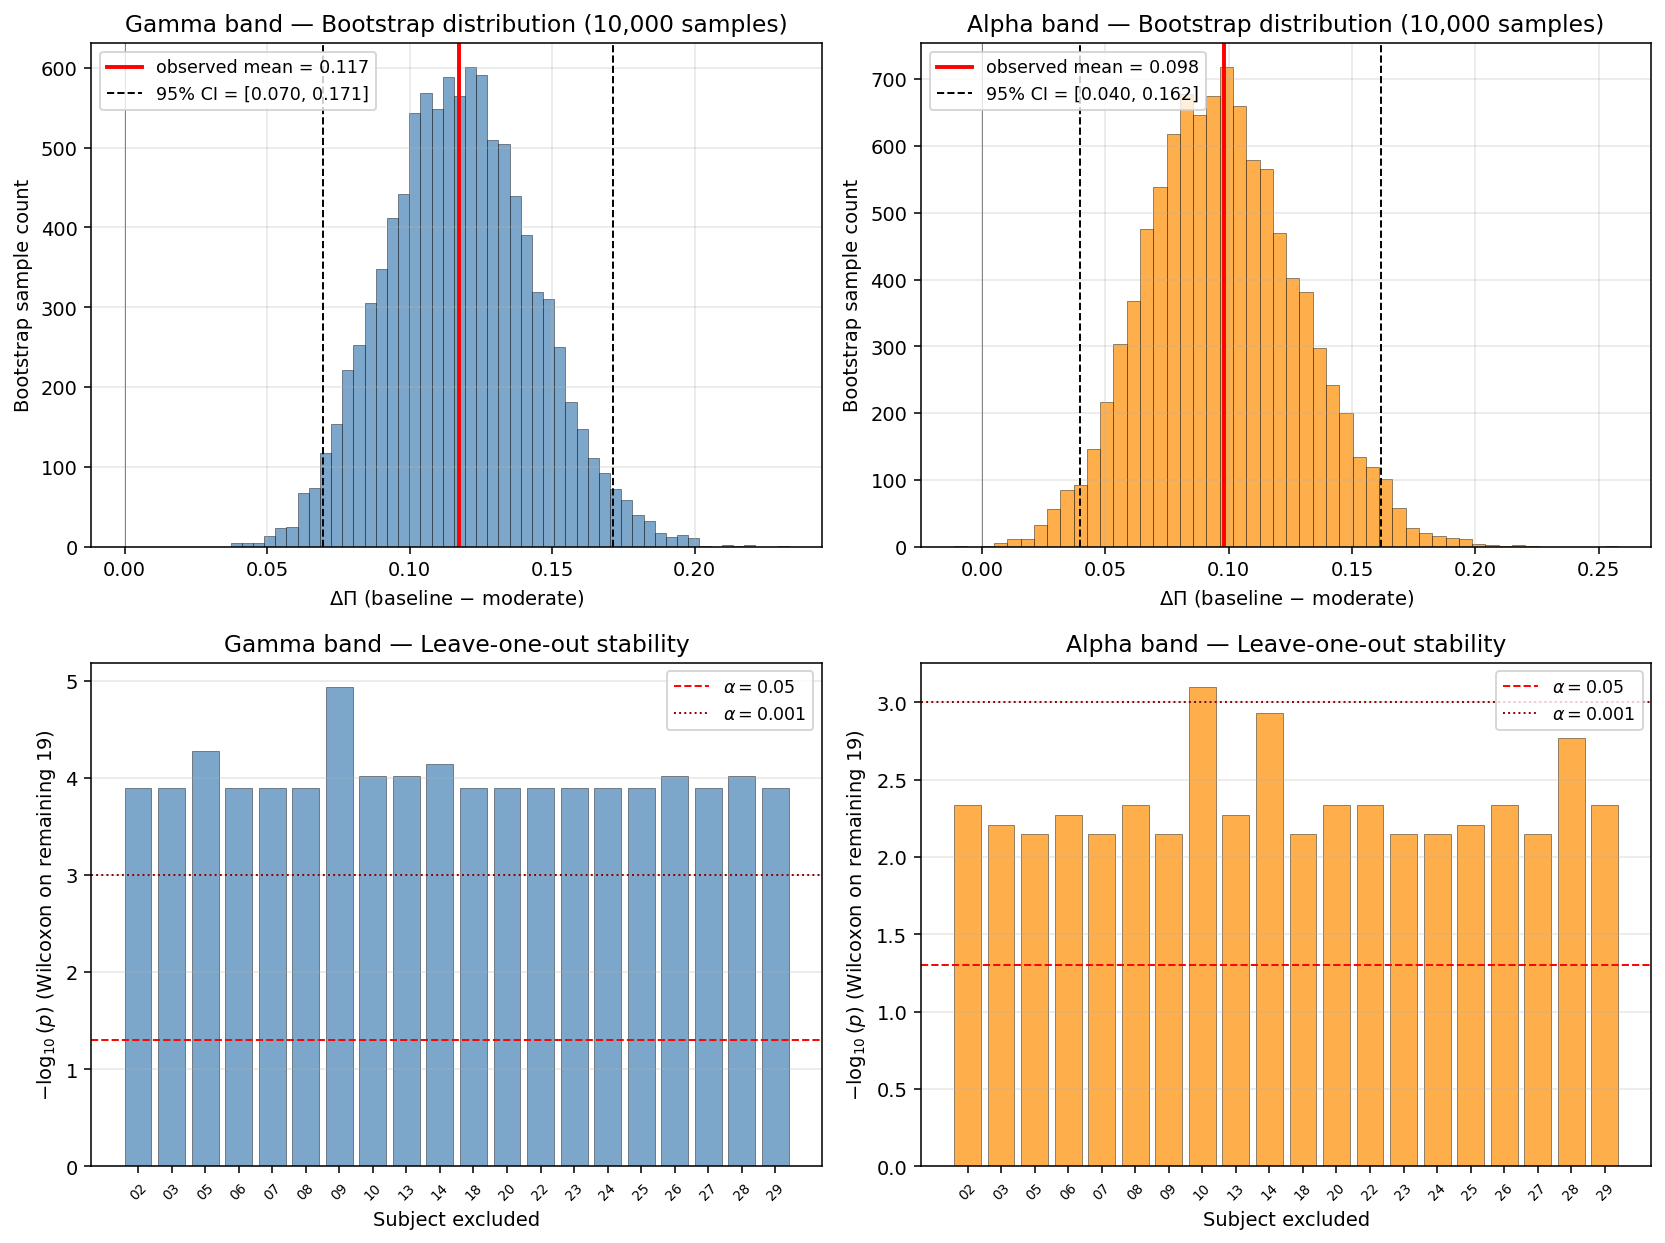
\includegraphics[width=0.95\linewidth]{pilot_robustness.png}
\caption{Robustness diagnostics for the pilot finding. Top: bootstrap distributions (10{,}000 resamples) of the mean $\Pi$-decline, gamma band (left) and alpha band (right). Bottom: leave-one-out $p$-values (Wilcoxon on the remaining 19 participants) as $-\log_{10}(p)$; both bands remain highly significant upon exclusion of any individual participant.}
\par\small\textbf{Alt text:} Robustness plots show bootstrap distributions of the sedation-related access-index decline and leave-one-out significance values, indicating that the main pilot effect is not driven by a single participant.\normalsize
\label{fig:pilot-robust}
\end{figure}

\paragraph{Sensitivity sweep over calibration hyperparameters.}
To quantify robustness against the methodological choice of calibration hyperparameters, we performed a full grid sweep: quantile width $\alpha \in \{0.05,\, 0.10,\, 0.15,\, 0.20\}$, $D_{\mathrm{eff}}$ window length $\tau_D \in \{0.1,\, 0.2,\, 0.4\}$~s, metastability window length $\tau_M \in \{0.3,\, 0.5,\, 1.0\}$~s --- i.e., 36 parameter combinations per band. For each combination, observables, per-participant calibration, and the Wilcoxon test on paired $\Pi$-values were recomputed.

The result (Figure~\ref{fig:pilot-sweep}): \emph{in the gamma band, all 36 of 36 parameter combinations reach $p < 10^{-3}$}, with $p$-values ranging from $2.67 \times 10^{-5}$ to $7.08 \times 10^{-4}$ and Cohen's~$d$ values between $0.91$ and $1.09$. The mean difference $\Delta\Pi$ varies between $0.070$ and $0.162$, but the sign of the effect is preserved in all configurations (100\,\% directional stability). In the alpha band, all 36 combinations reach $p < 0.05$, 33 of 36 reach $p < 0.01$, and 9 of 36 reach $p < 0.001$. Cohen's~$d$ varies between $0.62$ and $0.98$ (median $0.74$). The originally used parameters ($\alpha = 0.1$, $\tau_D = 0.2$~s, $\tau_M = 0.5$~s) lie in both bands in the intermediate range of observed effect sizes, not near an extremum.

\begin{figure}[h]
\centering
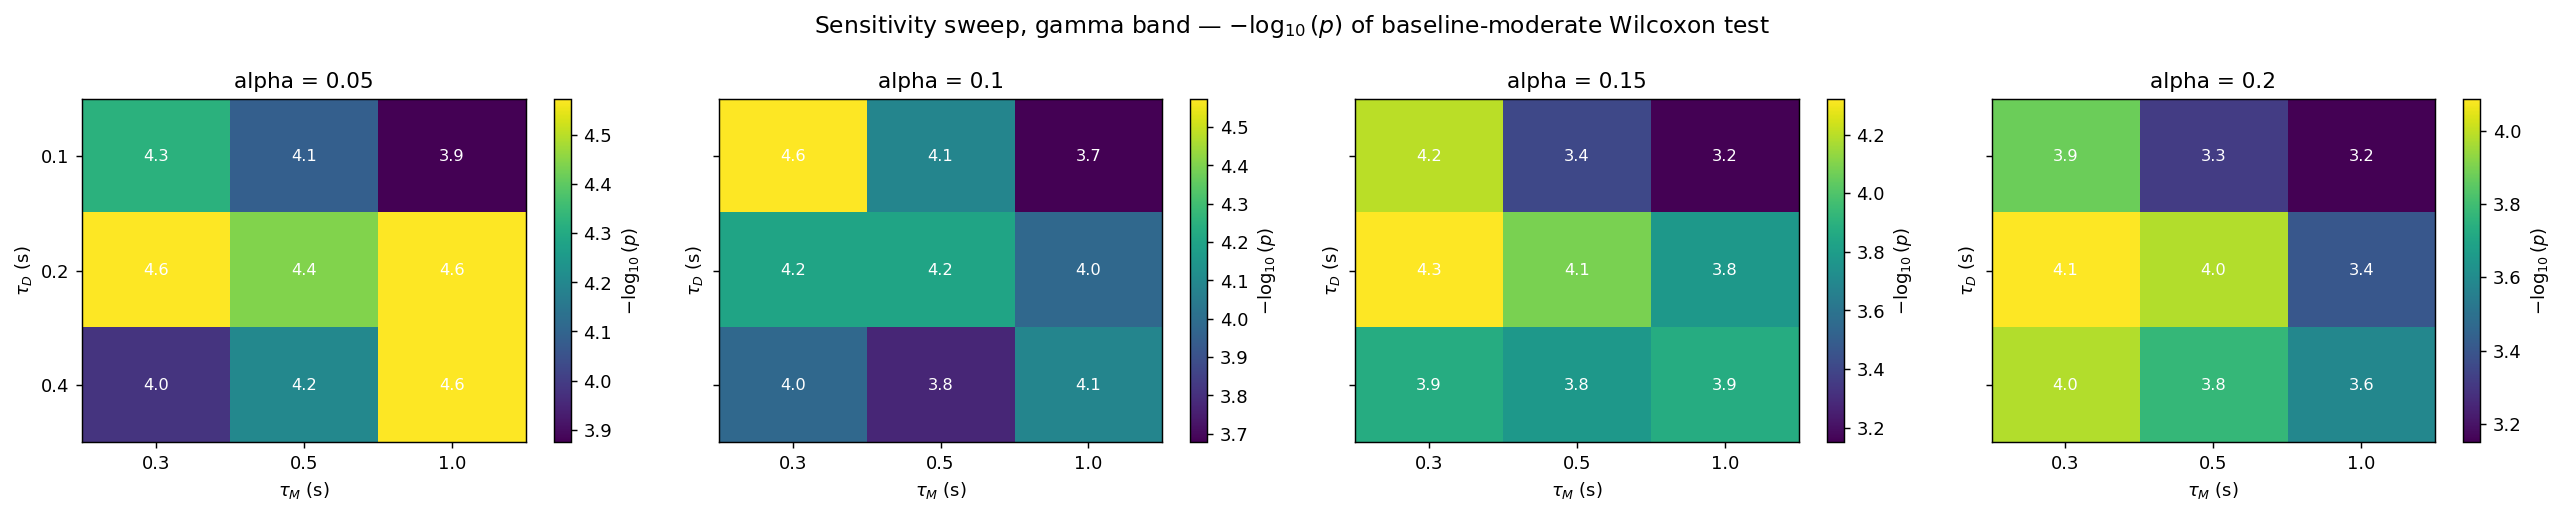
\includegraphics[width=0.98\linewidth]{sweep_heatmap_gamma.png}\\[0.3em]
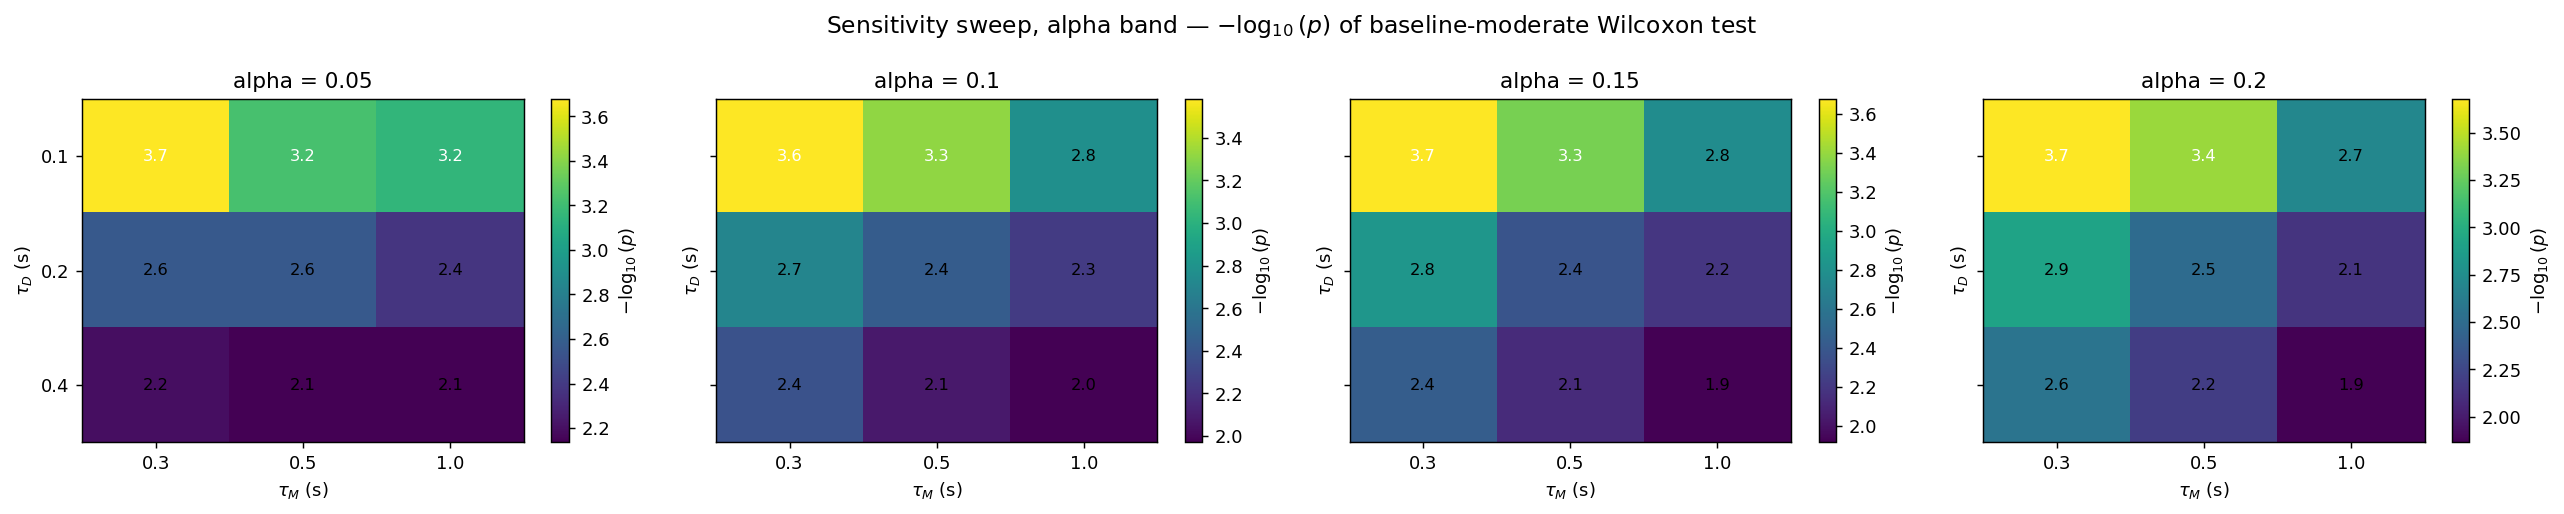
\includegraphics[width=0.98\linewidth]{sweep_heatmap_alpha.png}
\caption{Sensitivity sweep over calibration hyperparameters. Heatmaps of $-\log_{10}(p)$ for the baseline-vs-moderate Wilcoxon test, per $\alpha$ quantile value (panels), $\tau_D$ (rows), and $\tau_M$ (x-axis within each panel). Top: gamma band. Bottom: alpha band. All 72 combinations remain significant; the direction of the effect is never reversed.}
\par\small\textbf{Alt text:} Heatmaps across calibration choices show that baseline-versus-moderate sedation differences remain statistically significant across all tested quantiles and time-scale parameters in both gamma and alpha bands.\normalsize
\label{fig:pilot-sweep}
\end{figure}

\subsection{Template-Source Robustness: Chennu fsaverage Analysis}
\label{sec:source-robustness}

Because channel-level coherence can be inflated by volume conduction and reference effects, we repeated the Chennu baseline-vs-moderate comparison after an explicit template-source reconstruction. EEG sensors were assigned a combined standard-10--20/HydroCel montage, mapped to the MNE fsaverage template, projected with an sLORETA/minimum-norm inverse solution, and reduced to 68 cortical aparc ROIs \citep{gramfort2013,pascualmarqui2002}. This is not individualized MRI source localization. It is a source-level robustness check designed to ask whether the effect disappears once the analysis is moved away from raw sensor synchrony.

The direction survived. In alpha, source-space $\Pi$ declined from baseline $0.828$ to moderate sedation $0.781$ ($\Delta\Pi=0.0466$, 95\% CI $[0.0276,0.0670]$, paired $d_z=1.03$, one-sided Wilcoxon $p=1.94\times10^{-4}$). In gamma, source-space $\Pi$ declined from $0.828$ to $0.793$ ($\Delta\Pi=0.0342$, 95\% CI $[0.0098,0.0592]$, $d_z=0.59$, $p=0.0098$). Thus the Chennu effect passes the pre-specified robustness criterion for the alpha band ($p<0.01$, $d_z>0.5$) and remains directionally consistent and nominally significant in gamma (Figure~\ref{fig:central-evidence}A).

The interpretation remains deliberately narrow. This result does not remove all source-localization uncertainty, and it does not replace individualized head models or MEG/source-space replication. It does, however, neutralize the simplest sensor-level objection: the GCC decline is not lost when the Chennu analysis is recomputed on template-source ROI time series.

\subsection{Independent Replication: OpenNeuro DS005620}
\label{sec:ds005620}

To test whether the GCC effect generalizes beyond the Chennu dataset, we repeated the subject-calibrated analysis on OpenNeuro DS005620, a public repeated-awakening propofol EEG dataset with 21 healthy participants and BrainVision recordings at 5000~Hz \citep{bajwa2024ds005620}. We used the eyes-closed awake resting recording for within-subject calibration and compared it with the resting sedation conditions \texttt{sed} and \texttt{sed2}. For paired inference, participants with available awake and sedation recordings in the analysed subset were retained ($N=20$). The preprocessing and regime scoring followed the same logic as in Chennu: channel-level Hilbert phases, per-subject awake calibration, and subject-level paired comparison of $\Pi$.

The replication is directionally and statistically strong. In the gamma band, $\Pi$ declined from awake to \texttt{sed} by $\Delta\Pi = 0.387$ (95\% CI $[0.305,0.479]$, paired $d=1.91$, FDR-corrected sign-flip $q=1.0\times10^{-4}$) and from awake to \texttt{sed2} by $\Delta\Pi = 0.341$ (95\% CI $[0.267,0.416]$, $d=1.97$, $q=1.0\times10^{-4}$). In the alpha band, the corresponding effects were smaller but still robust: awake vs.\ \texttt{sed}, $\Delta\Pi = 0.177$ (95\% CI $[0.112,0.242]$, $d=1.16$, $q=1.5\times10^{-4}$); awake vs.\ \texttt{sed2}, $\Delta\Pi = 0.164$ (95\% CI $[0.099,0.229]$, $d=1.08$, $q=1.8\times10^{-4}$).

A local audit against the OpenNeuro file manifest confirmed that the analysed subset contains the complete resting-state core used for this comparison: 21 eyes-closed awake recordings, 54 \texttt{sed} resting recordings, and 51 \texttt{sed2} resting recordings. The remaining public DS005620 recordings not included here are eyes-open awake and TMS acquisitions rather than missing resting sedation files. To reduce the possibility that the effect is driven by choosing unusually separable sedation runs, we repeated the comparison using, for each participant and target state, the sedated run closest to awake in a standardized spectral-feature space (theta, alpha, beta, gamma power, alpha/gamma ratio, spectral entropy). The effect survived this conservative run-selection rule (gamma awake-vs-\texttt{sed}: $\Delta\Pi=0.360$, 95\% CI $[0.263,0.461]$, $d=1.58$, AUC $=1.00$; alpha awake-vs-\texttt{sed}: $\Delta\Pi=0.176$, 95\% CI $[0.104,0.246]$, $d=1.05$, AUC $=0.80$).

Pooling the six subject-level EEG cells across Chennu and DS005620 yields a mean $\Delta\Pi = 0.214$ over 120 paired subject-cell observations (bootstrap 95\% CI $[0.181,0.249]$, paired $d=1.12$, sign-flip $p=5.0\times10^{-5}$). A participant-cluster bootstrap over 40 participant identifiers gives a more conservative estimate of $0.187$ (95\% CI $[0.148,0.228]$; Wilcoxon over participant means $p=5.0\times10^{-11}$). These values support the narrow empirical claim that subject-calibrated GCC regime occupancy is a reproducible marker of sedation-related state change across two independent public EEG datasets.

The larger DS005620 effect should not be interpreted as a universal effect-size estimate. The two datasets differ in acquisition and protocol: Chennu used 91-channel EEG sampled at 250~Hz across four pharmacological stages including mild and recovery states, whereas DS005620 used BrainVision recordings sampled at 5000~Hz in a repeated-awakening propofol paradigm and, in the present analysis, an eyes-closed awake calibration against resting sedation recordings. These differences can affect signal-to-noise ratio, vigilance stability, spectral structure, and calibration sharpness. The replication therefore supports \emph{directional reproducibility} of the GCC state effect, not equality of absolute effect sizes across datasets. The very large DS005620 AUC values reported below are consequently treated as dataset-specific separability under the present preprocessing and subject-level calibration, not as evidence that perfect classification should generalize to other propofol cohorts.

\subsection{Spectral Baselines, Frozen Transfer, and Lagged-Coupling Controls}
\label{sec:spectral-controls}

Because sedation EEG is strongly reflected in spectral power, GCC was benchmarked against subject-normalized theta, alpha, beta, gamma, alpha/gamma ratio, and spectral entropy features. Raw gamma $\Pi$ was a strong state marker within Chennu (AUC $=0.87$) and DS005620 (AUC $=1.00$), but bandpower residualization reduced performance (AUC $=0.61$ and $0.68$). Cross-dataset residual transfer was asymmetric (Chennu$\to$DS005620 AUC $=0.93$; DS005620$\to$Chennu AUC $=0.30$), likely reflecting differences in acquisition, calibration, state depth, and spectral signal-to-noise. We therefore do not claim that GCC is generally bandpower-independent. The defensible claim is narrower: GCC is a reproducible subject-calibrated regime composite whose information partly overlaps with conventional spectral state markers.

Artifact and coupling controls constrain the interpretation further. In DS005620, the gamma effect survived posterior and centro-posterior channel restrictions ($\Delta\Pi\approx0.21$, AUC $=0.95$--$1.00$), whereas posterior 70--110~Hz power did not distinguish awake from sedation (AUC $=0.53$) and did not correlate with posterior $\Pi$ change. Phase-randomized surrogates did not eliminate separation, showing that channel-level GCC still carries univariate spectral state information. However, replacing zero-lag-sensitive coherence with a wPLI-style lagged-coupling proxy retained sedation sensitivity in both datasets \citep{vinck2011}: DS005620 gamma AUCs were $0.90$--$0.91$ on spectrally closest runs, and Chennu gamma/alpha AUCs were $0.77$ and $0.90$.

Finally, a frozen cross-dataset benchmark used either a no-fit sign rule or train-on-one-dataset/test-on-the-other logistic transfer (Supplementary Table S5). Standard gamma $\Pi$ generalized strongly (pooled no-fit AUC $=0.967$; Chennu$\to$DS005620 AUC $=1.00$; DS005620$\to$Chennu AUC $=0.90$). The lagged-coupling triad plus $\Pi$ also generalized bidirectionally (AUC $=0.95$ and $0.90$). Spectral bandpowers remained highly competitive, so the benchmark strengthens reproducibility and artifact resistance, not spectral independence.


\subsection{Non-Propofol State Check: Sleep-EDF}
\label{sec:sleep-edf}

To test whether the GCC observable geometry is restricted to propofol sedation, we applied the frozen feature pipeline to an expanded local subset of the Sleep-EDF Sleep Cassette dataset from PhysioNet \citep{kemp2000}. The analysed subset contained 22 PSG--hypnogram recordings, 23,235 scored 30~s epochs, and three coarse states: Wake, REM, and NREM. Because Sleep-EDF provides only two EEG channels in this configuration (\texttt{EEG Fpz-Cz} and \texttt{EEG Pz-Oz}), this analysis is not a large-scale network validation and not a direct test of conscious access. It is used only as a non-propofol state-differentiation check of the GCC observables.

We evaluated the sleep-relevant sigma band (12--16~Hz) with the same quantile-calibrated regime logic ($\alpha=0.10$), using Wake epochs as the reference distribution. Under leave-recording-out validation, conventional spectral features remained the strongest sleep-stage markers. The GCC triad plus $\Pi$ nevertheless separated Wake from NREM with AUC $=0.875$ and REM from NREM with AUC $=0.727$ (Figure~\ref{fig:central-evidence}C; Supplementary Table S6). $\Pi$ alone was weak in both contrasts (AUC $\approx0.534$), which is scientifically important: the empirical sleep result supports a multivariate regime-geometry interpretation, not a scalar $\Pi$-only sleep biomarker.


At the subject/recording level, $\Pi$ was higher in Wake than NREM (mean $\Delta\Pi=0.0427$, $d_z=0.793$, Wilcoxon $p=0.00145$) and higher in REM than NREM (mean $\Delta\Pi=0.0517$, $d_z=0.949$, $p=0.000256$). The metastability observable $M_\tau$ showed the same qualitative direction (REM--NREM: $d_z=0.855$, $p=0.00126$). The interpretation is deliberately conservative. Sleep-EDF adds a third public state-transition domain and shows that the GCC observables are not exclusively propofol-sensitive. However, two-channel sleep staging cannot adjudicate the access claim itself, REM is not equivalent to waking access, and sigma-band sleep physiology differs from gamma-band propofol dynamics. The result therefore strengthens the general state-geometry claim, but not the clinical selective-preservation extension.

\subsection{Public Disorders-of-Consciousness Pilot Anchor}
\label{sec:doc-anchor}

To add a clinical anchor outside healthy pharmacological state modulation, we analysed a public EEG/PSG disorders-of-consciousness dataset from Mendeley Data (DOI: \href{https://doi.org/10.17632/6wx4n25h4v.1}{10.17632/6wx4n25h4v.1}). The local audit identified 42 EDF files: 30 vegetative-state/unresponsive-wakefulness-syndrome (VS/UWS) recordings, 4 MCS- recordings, and 8 MCS+ recordings. The primary endpoint was pre-specified as alpha-band subject-calibrated GCC access $\Pi$ for MCS+ versus VS, using the common six-channel montage F3, F4, C3, C4, O1, and O2. Because this dataset is small and class-imbalanced, it is treated as a pilot clinical anchor rather than as a definitive diagnostic validation.

The pre-specified primary endpoint was statistically significant in its unadjusted form but marginal under correction across the broader exploratory family. Raw alpha-band $\Pi$ distinguished MCS+ from VS with AUC $=0.754$ (bootstrap 95\% CI $[0.579,0.900]$), mean difference $0.197$, and label-permutation AUC $p=0.017$. After residualizing conventional spectral features, the AUC remained $0.717$ (95\% CI $[0.529,0.879]$, permutation $p=0.027$). After residualizing both spectral features and retained artifact-clean epochs, the AUC was $0.721$ (95\% CI $[0.533,0.883]$, permutation $p=0.017$; Figure~\ref{fig:central-evidence}D). Across the full exploratory alpha-threshold/band/contrast/score family, the primary Benjamini--Hochberg q-value was approximately $0.084$; within score families, q-values were approximately $0.064$--$0.092$. This pattern is consistent with a pilot clinical anchor, not with definitive diagnostic validation.

The clinical reading is therefore narrow but useful. The DoC result shows that GCC carries pilot signal in the expected direction in a severe clinical population and that the primary effect survives label permutation and spectral/epoch-count residualization. It does not establish GCC as a diagnostic biomarker, does not validate selective-preservation re-entry, and should not be used to claim clinical readiness. Its role in the present manuscript is to answer a more limited reviewer question: whether GCC remains operationally meaningful outside healthy propofol and sleep-state datasets.

\subsection{Additional Robustness and Boundary-Domain Analyses}
\label{sec:additional-controls}

Four additional analyses reduce implementation-specific degrees of freedom. An amplitude-normalized phase-only pipeline retained propofol sensitivity without entering bandpass amplitude directly into $R$, $\Deff$, or $\Mtau$ (Chennu gamma $\Delta\Pi=0.463$, $d=2.37$; DS005620 gamma $\Delta\Pi=0.439$, $d=1.99$). A current-source-density surface-Laplacian source-proxy also retained the effect (Chennu gamma $\Delta\Pi=0.159$, $d=1.12$; DS005620 gamma $\Delta\Pi=0.393$, $d=1.67$).

Two boundary-domain datasets tested breadth rather than direct access validation. In public subanaesthetic ketamine data \citep{farnes2020}, gamma $\Pi$ shifted downward ($0.830$ to $0.688$, $d=-1.09$, $p=0.0098$) while alpha $\Deff$ increased, consistent with an altered-state geometry rather than propofol-like loss of consciousness. In OpenNeuro DS004504 \citep{miltiadous2023ds004504}, combined alpha/gamma GCC features separated dementia-proxy participants from controls (AUC $=0.769$, balanced accuracy $=0.786$), and alpha $R$ and $\Deff$ correlated with MMSE. These analyses broaden the empirical interface but do not test residual-backbone re-entry.


To reduce post-hoc flexibility, the final public-feature analyses were also documented in a frozen validation specification before being integrated into the manuscript. The frozen pipeline fixes the primary phase-only implementation, bands, window length, stride, quantile calibration, mandatory spectral baselines, source-proxy controls, and forbidden claims. This does not make the present analyses preregistered in the formal sense, but it provides a locked template for prospective external validation.

\subsection{From Ensemble Semantics to Per-Subject Application: A Working Assumption}
\label{sec:pilot-bridge}

In the simulations, $\Pi$ is an ensemble quantity; in the EEG analyses, it is calibrated within one participant's baseline recording. The bridge rests on an ergodicity-type working assumption: a sufficiently long recording under stable conditions approximates effective ensemble averaging. This assumption is not derived from the model. The two propofol datasets, split-half checks, and repeated-run analyses support its practical use, but a formal validation would require recording-duration tests and independent baseline sessions.

\subsection{Limits and Caveats}
\label{sec:pilot-limits}

The public EEG validation has five main limits. First, baseline $\Pi$ is close to $0.66$ by construction under the per-subject quantile calibration; only deviations from baseline are interpretable. Second, the primary analysis is channel-level. wPLI, CSD/surface-Laplacian, and template-source checks reduce but do not remove the need for individualized source reconstruction or MEG. Third, Hilbert phases of EEG channels are only an approximation to the oscillator phases in the theoretical model. Fourth, DS005620 yields larger raw effects than Chennu, and residualized transfer is asymmetric, plausibly because acquisition, channel layout, state depth, and calibration differ. Fifth, bandpower residualization and phase-randomized surrogates show substantial overlap with conventional spectral state markers; GCC is not claimed as a bandpower-independent biomarker.

Most importantly, the present data do not directly test P1. Propofol and ketamine involve pharmacological state modulation in healthy participants; the DoC and DS004504 analyses provide clinical and degradation-proxy anchors but not longitudinal selective-preservation re-entry. A direct P1 validation would require structurally degraded cohorts with repeated access markers, longitudinal recordings, and evidence for residual-backbone/gain redistribution. Thus the present work establishes operational state sensitivity and model-internal mechanism, not the full clinical re-entry claim.


% ==================================================================
% ==================================================================
% ========================= DISCUSSION =============================
% ==================================================================
\fi
\section*{Discussion}
\addcontentsline{toc}{section}{Discussion}

\noindent\textit{The following sections discuss the relative originality of the GCC framework, the main discussion and interpretation of the findings, and a concluding summary with explicit boundaries of what the present work delivers and what it does not.}

% ==================================================================
\section{Relative Originality}
\label{sec:originalitaet}

The GCC claims no absolute monopoly on its components. Integration, synchrony, critical dynamics, global availability, and metastability are each well established in the literature \citep{dehaene1998,tononi2004,fries2015,deco2017}. The relative distinctive feature lies in their explicit assembly into a single operational regime model for access-compatible neural dynamics, evaluated through a prediction family over nonlinear transitions, degradation shifts, bounded access intervals, anesthesia-like trajectories, and selective-preservation re-entry in controlled simulations. The clinical degradation hypothesis is an extension of this regime framework, not the sole foundation of the manuscript.

% ==================================================================
\section{Discussion}
\label{sec:diskussion}

The main claim evaluated in this paper is that access-compatible dynamics occupy a bounded, calibrated regime rather than increasing monotonically with any single observable. The empirical part now supports this claim at the level appropriate for a principled computational model: GCC regime occupancy can be computed from real EEG, decreases reproducibly under propofol sedation across two independent public datasets, survives a gamma-band topographic artifact stress test, persists under spectrally closest run selection, transfers under frozen train-on-one-dataset/test-on-the-other rules, and remains present when zero-lag-sensitive coherence is replaced by a wPLI-style lagged-coupling proxy. At the same time, the spectral residualization, phase-surrogate, and spectral-baseline results impose an important boundary: GCC is not established here as a bandpower-independent biomarker, and conventional bandpowers remain strong competitors. It should be interpreted as a multi-observable regime composite whose condition information partly overlaps with conventional spectral state markers. Embedded in the broader framework of balanced consensus formation, the strongest empirically defended reading of the model is:

\begin{quote}
\itshape
Level of consciousness and global access are favored in a critical dynamical regime in which residual network topology, effective gain structure, noise, and delays jointly produce sufficient but non-rigid macroscopic integration.
\end{quote}

The counterintuitive degradation extension is narrower: functional re-integration in damaged systems may arise from selective preservation and gain redistribution, not only from increased global activity. The present work supports this statement as a controlled model-internal mechanism. It does not establish it in structurally degraded biological cohorts, and it should not be presented as an empirical result about terminal lucidity or disorders of consciousness.

\subsection{Future Directions}
\label{sec:future-directions}

The most important next step is not a stronger philosophical claim but a stricter empirical test. Three developments would directly strengthen or falsify the GCC. First, regime boundaries should be calibrated out of sample across heterogeneous EEG/MEG cohorts. Second, template-source robustness should be replaced by individualized source-level EEG/MEG or intracranial recordings where possible. Third, selective preservation should be tested prospectively in structurally degraded clinical cohorts with repeated behavioral access measures and longitudinal recordings.

% ==================================================================
\section{Conclusion}
\label{sec:schluss}

The GCC is not a full model of consciousness but a consistent, operationalized, and testable principled model of access-compatible neural dynamics. Its present status is strongest as a regime model evaluated by simulations and public EEG validation: the observables are computable, state-sensitive, reliable at recording level, and capable of expressing bounded access rather than monotonic coherence. Across two independent public propofol datasets, subject-calibrated GCC regime occupancy declines reproducibly under sedation, and the Chennu effect survives a template-source ROI robustness check. Sleep-EDF, a public DoC EEG/PSG dataset, ketamine, and dementia-proxy analyses add boundary-domain checks in which the GCC geometry differentiates sleep states, carries a pilot clinical MCS+ vs VS signal, shifts under altered conscious pharmacology, and captures neurodegenerative group structure without being overinterpreted as direct access validation. The empirical result is strengthened by subject-level confidence intervals, FDR/permutation transparency, frozen cross-dataset transfer, spectrally closest run controls, gamma artifact controls, a wPLI-based lagged-coupling stress test, amplitude-normalized phase-only GCC, CSD/source-proxy GCC, template-source robustness, reliability analyses, and a frozen validation specification; it is limited by substantial overlap with conventional spectral bandpower, mostly channel-level measurement, small clinical samples, and the absence of a direct P1 clinical re-entry dataset. Its principal theoretical move remains the separation of topology and functional efficacy through the gain model. The selective-preservation account of re-entry in structurally degraded systems remains a clinical extension and future empirical target, not the central validated result of the present paper.


% ==================================================================
\newpage
\section*{Acknowledgments}
\addcontentsline{toc}{section}{Acknowledgments}

The author thanks the Chennu et al.\ (2016) team, the DS005620/OpenNeuro contributors, the PhysioNet/Sleep-EDF contributors, the Mendeley disorders-of-consciousness dataset contributors, the Farnes et al.\ ketamine-data contributors, and the DS004504/OpenNeuro contributors for making their EEG datasets publicly available, which made the empirical validation analyses in this study possible. AI-assisted tools were used for programming support, language editing, and workflow organization; the author verified the analyses, controlled the scientific interpretation, and takes full responsibility for the content of the manuscript.

% ==================================================================
\section*{Funding}
\addcontentsline{toc}{section}{Funding}

No external funding was received for this work.

% ==================================================================
\section*{Author Contributions}
\addcontentsline{toc}{section}{Author Contributions}

Mehmet Oktay Tugan: Conceptualization, methodology, software, formal analysis, investigation, validation, visualization, writing--original draft, writing--review and editing.

% ==================================================================
\section*{Ethics Statement}
\addcontentsline{toc}{section}{Ethics Statement}

This study is a secondary analysis of publicly available, de-identified human EEG datasets and synthetic simulations. No new human participants were recruited and no new human or animal data were collected. Ethical approvals and informed consent were obtained by the original data-generating studies where applicable. No additional institutional ethics approval was required for the present secondary analysis.

% ==================================================================
\section*{Data Availability}
\addcontentsline{toc}{section}{Data Availability}

The re-analysed datasets are publicly available: Chennu et al.\ EEG \citep{chennu2016} (DOI: \href{https://doi.org/10.17863/CAM.68959}{10.17863/CAM.68959}), OpenNeuro DS005620 \citep{bajwa2024ds005620}, Sleep-EDF Sleep Cassette \citep{kemp2000}, the Mendeley disorders-of-consciousness EEG/PSG dataset (DOI: \href{https://doi.org/10.17632/6wx4n25h4v.1}{10.17632/6wx4n25h4v.1}), the Farnes et al.\ ketamine EEG data \citep{farnes2020}, and OpenNeuro DS004504 \citep{miltiadous2023ds004504}. Raw third-party datasets are not redistributed. Author-generated simulation code, analysis scripts, derived result tables, figures, and reproducibility instructions are provided in the public GCC reproducibility repository at \url{https://github.com/oktaytugan82/gcc_simulation}. The NoC preflight-clean submission package is archived as release \texttt{v2.0.1-noc-preflight} on Zenodo (version DOI: \href{https://doi.org/10.5281/zenodo.19818741}{10.5281/zenodo.19818741}; concept DOI for the latest repository version: \href{https://doi.org/10.5281/zenodo.19744969}{10.5281/zenodo.19744969}).

% ==================================================================
\section*{Competing Interests}
\addcontentsline{toc}{section}{Competing Interests}

The author has declared that no competing interests exist.

% ==================================================================
\section*{Supplementary Material}
\addcontentsline{toc}{section}{Supplementary Material}

Supplementary Text S1 contains the mathematical well-posedness results, observable bounds, finite-horizon stability estimates, the sufficient selective-preservation re-entry condition, and the discussion of Gronwall conservativity. Supplementary code and derived analysis outputs are provided in the reproducibility package described in the Data Availability statement.

% ==================================================================

% ==================================================================
\section*{Supporting Information}
\addcontentsline{toc}{section}{Supporting Information}

\noindent\textbf{S1 Code. GCC simulation and analysis code} (\texttt{gcc\_simulation\_v2.0.1-noc-preflight.zip})\textbf{.} Complete Python codebase for the GCC dynamical model, per-subject EEG analysis pipeline, ensemble simulations, retuning-control sweep, sweep-level statistical analysis, spectral baseline comparison, bandpower residualization, DS005620 replication, gamma artifact-control scripts, phase-surrogate controls, wPLI lagged-coupling controls, frozen cross-dataset benchmarks, amplitude-normalized phase-only GCC, CSD/source-proxy GCC, template-source Chennu robustness analysis, Sleep-EDF state-differentiation analysis, public DoC pilot analysis, ketamine boundary-state analysis, DS004504 degradation-proxy analysis, split-half/repeated-run reliability analysis, frozen validation specification, and figure-generation scripts. Includes reproducibility instructions, derived result tables, manuscript source files, and the Batch~3--18 validation outputs reported here. The public repository is \url{https://github.com/oktaytugan82/gcc_simulation}; the NoC preflight-clean submission snapshot is release \texttt{v2.0.1-noc-preflight}, archived on Zenodo with version DOI \href{https://doi.org/10.5281/zenodo.19818741}{10.5281/zenodo.19818741}.


% ==================================================================
\newpage
\begin{thebibliography}{99}

\bibitem[Bajwa et~al.(2024)]{bajwa2024ds005620}
Bajwa,~I.\,J., Nilsen,~A.\,S., Skukies,~R., Aamodt,~A., Ernst,~G., Storm,~J.\,F., \& Juel,~B.\,E.\ (2024).
A repeated awakening study exploring the capacity of complexity measures to capture dreaming during propofol sedation.
\textit{OpenNeuro Dataset DS005620}.
\url{https://doi.org/10.18112/openneuro.ds005620.v1.0.0}


\bibitem[Chennu et~al.(2016)]{chennu2016}
Chennu,~S., O'Connor,~S., Adapa,~R., Menon,~D.\,K., \& Bekinschtein,~T.\,A.\ (2016).
Brain connectivity dissociates responsiveness from drug exposure during propofol-induced transitions of consciousness.
\textit{PLoS Computational Biology}, \textbf{12}(1), e1004669.
\url{https://doi.org/10.1371/journal.pcbi.1004669}

\bibitem[Casali et~al.(2013)]{casali2013}
Casali,~A.\,G., Gosseries,~O., Rosanova,~M., Boly,~M., Sarasso,~S., Casali,~K.\,R., Casarotto,~S., Bruno,~M.-A., Laureys,~S., Tononi,~G., \& Massimini,~M.\ (2013).
A theoretically based index of consciousness independent of sensory processing and behavior.
\textit{Science Translational Medicine}, \textbf{5}(198), 198ra105.
\url{https://doi.org/10.1126/scitranslmed.3006294}

\bibitem[Deco et~al.(2017)]{deco2017}
Deco,~G., Kringelbach,~M.\,L., Jirsa,~V.\,K., \& Ritter,~P.\ (2017).
The dynamics of resting fluctuations in the brain: Metastability and its dynamical cortical core.
\textit{Scientific Reports}, \textbf{7}, 3095.
\url{https://doi.org/10.1038/s41598-017-03073-5}

\bibitem[Dehaene et~al.(1998)]{dehaene1998}
Dehaene,~S., Kerszberg,~M., \& Changeux,~J.-P.\ (1998).
A neuronal model of a global workspace in effortful cognitive tasks.
\textit{PNAS}, \textbf{95}(24), 14529--14534.
\url{https://doi.org/10.1073/pnas.95.24.14529}

\bibitem[Demertzi et~al.(2019)]{demertzi2019}
Demertzi,~A., Tagliazucchi,~E., Dehaene,~S., Deco,~G., Barttfeld,~P., Raimondo,~F., Martial,~C., Fernandez-Espejo,~D., Rohaut,~B., Voss,~H.\,U., Schiff,~N.\,D., Owen,~A.\,M., Laureys,~S., Naccache,~L., Sitt,~J.\,D., \& Chennu,~S.\ (2019).
Human consciousness is supported by dynamic complex patterns of brain signal coordination.
\textit{Science Advances}, \textbf{5}(2), eaat7603.
\url{https://doi.org/10.1126/sciadv.aat7603}

\bibitem[Engemann et~al.(2018)]{engemann2018}
Engemann,~D.\,A., Raimondo,~F., King,~J.-R., Rohaut,~B., Louppe,~G., Faugeras,~F., Annen,~J., Cassol,~H., Gosseries,~O., Fernandez-Slezak,~D., Laureys,~S., Naccache,~L., Dehaene,~S., \& Sitt,~J.\,D.\ (2018).
Robust EEG-based cross-site and cross-protocol classification of states of consciousness.
\textit{Brain}, \textbf{141}(11), 3179--3192.
\url{https://doi.org/10.1093/brain/awy251}

\bibitem[Fries(2015)]{fries2015}
Fries,~P.\ (2015).
Rhythms for cognition: Communication through coherence.
\textit{Neuron}, \textbf{88}(1), 220--235.
\url{https://doi.org/10.1016/j.neuron.2015.09.034}

\bibitem[Farnes et~al.(2020)]{farnes2020}
Farnes,~N., Juel,~B.\,E., Nilsen,~A.\,S., Romundstad,~L.\,G., \& Storm,~J.\,F.\ (2020).
Increased signal diversity/complexity of spontaneous EEG, but not evoked EEG responses, in ketamine-induced psychedelic state in humans.
\textit{PLoS ONE}, \textbf{15}(11), e0242056.
\url{https://doi.org/10.1371/journal.pone.0242056}


\bibitem[Kemp et~al.(2000)]{kemp2000}
Kemp,~B., Zwinderman,~A.\,H., Tuk,~B., Kamphuisen,~H.\,A.\,C., \& Oberye,~J.\,J.\,L.\ (2000).
Analysis of a sleep-dependent neuronal feedback loop: The slow-wave microcontinuity of the EEG.
\textit{IEEE Transactions on Biomedical Engineering}, \textbf{47}(9), 1185--1194.
\url{https://doi.org/10.1109/10.867928}

\bibitem[Mashour et~al.(2020)]{mashour2020}
Mashour,~G.\,A., Roelfsema,~P., Changeux,~J.-P., \& Dehaene,~S.\ (2020).
Conscious processing and the global neuronal workspace hypothesis.
\textit{Neuron}, \textbf{105}(5), 776--798.
\url{https://doi.org/10.1016/j.neuron.2020.01.026}

\bibitem[Miltiadous et~al.(2023)]{miltiadous2023ds004504}
Miltiadous,~A., Tzimourta,~K.\,D., Afrantou,~T., Ioannidis,~P., Grigoriadis,~N., Tsalikakis,~D.\,G., Angelidis,~P., Tsipouras,~M.\,G., Glavas,~E., Giannakeas,~N., \& Tzallas,~A.\,T.\ (2023).
A dataset of EEG recordings from: Alzheimer's disease, frontotemporal dementia and healthy subjects.
\textit{OpenNeuro Dataset DS004504}.
\url{https://doi.org/10.18112/openneuro.ds004504.v1.0.8}


\bibitem[Sitt et~al.(2014)]{sitt2014}
Sitt,~J.\,D., King,~J.-R., El~Karoui,~I., Rohaut,~B., Faugeras,~F., Gramfort,~A., Cohen,~L., Sigman,~M., Dehaene,~S., \& Naccache,~L.\ (2014).
Large scale screening of neural signatures of consciousness in patients in a vegetative or minimally conscious state.
\textit{Brain}, \textbf{137}(8), 2258--2270.
\url{https://doi.org/10.1093/brain/awu141}


\bibitem[Restrepo et~al.(2005)]{restrepo2005}
Restrepo,~J.\,G., Ott,~E., \& Hunt,~B.\,R.\ (2005).
Onset of synchronization in large networks of coupled oscillators.
\textit{Physical Review E}, \textbf{71}(3), 036151.
\url{https://doi.org/10.1103/PhysRevE.71.036151}


\bibitem[Tononi(2004)]{tononi2004}
Tononi,~G.\ (2004).
An information integration theory of consciousness.
\textit{BMC Neuroscience}, \textbf{5}, 42.
\url{https://doi.org/10.1186/1471-2202-5-42}

\bibitem[Vinck et~al.(2011)]{vinck2011}
Vinck,~M., Oostenveld,~R., van Wingerden,~M., Battaglia,~F., \& Pennartz,~C.\,M.\,A.\ (2011).
An improved index of phase-synchronization for electrophysiological data in the presence of volume-conduction, noise and sample-size bias.
\textit{NeuroImage}, \textbf{55}(4), 1548--1565.
\url{https://doi.org/10.1016/j.neuroimage.2011.01.055}


\end{thebibliography}

\end{document}
